\Chapter{Multi-Agent Deep Reinforcement Learning in the context of Robotics}{Bridging the gap between MADRL research and robotics}
\label{ChapterMADRL} 




% Figure multi-agent environments (prisonner's dilemma -> pred-prey/foraging -> Hanabi -> SMAC/Dota -> Multi-robot warehouse -> HRI)
\begin{figure}[h]
    \centering
    \begin{subfigure}[c]{0.24\textwidth}
        \centering
        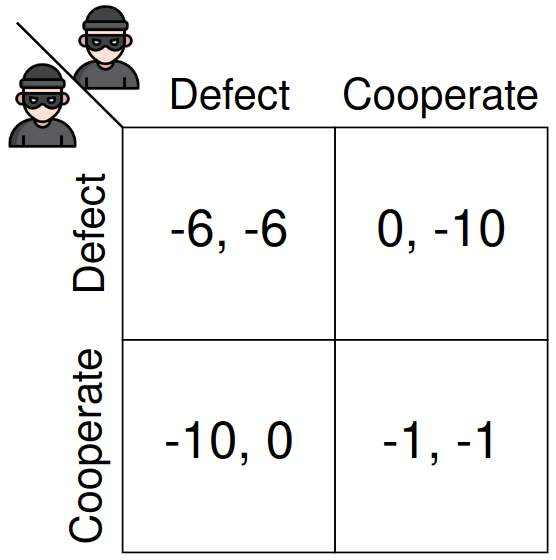
\includegraphics[width=\textwidth]{Figures/MADRL/prisonersdilema.png}
        \caption{Social dilemma}
        \label{fig:prisoners}
    \end{subfigure}
    \hfill
    \begin{subfigure}[c]{0.23\textwidth}
        \centering
        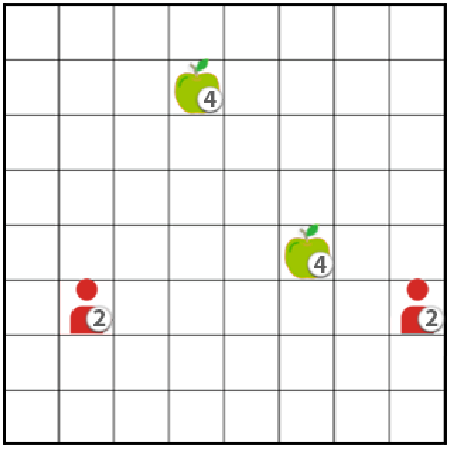
\includegraphics[width=\textwidth]{Figures/MADRL/lbf.png}
        \caption{Two-dimensional grid world}
        \label{fig:lbf1}
    \end{subfigure}
    \hfill
    \begin{subfigure}[c]{0.4\textwidth}
        \centering
        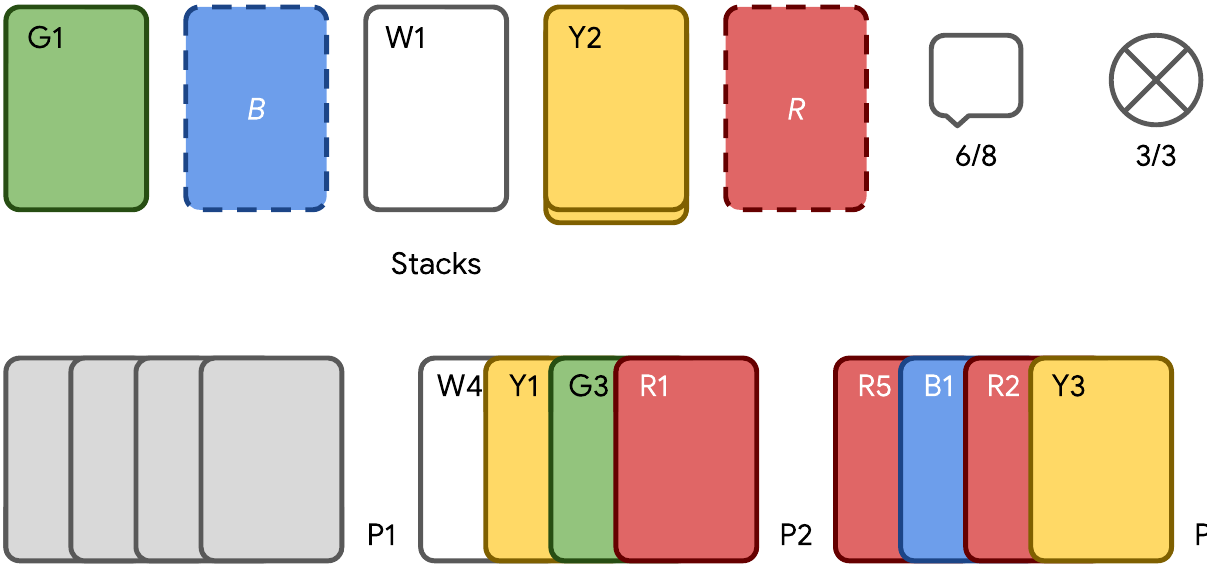
\includegraphics[width=\textwidth]{Figures/MADRL/hanabi.png}
        \caption{Card game}
    \end{subfigure}
    
    \begin{subfigure}[c]{0.32\textwidth}
        \centering
        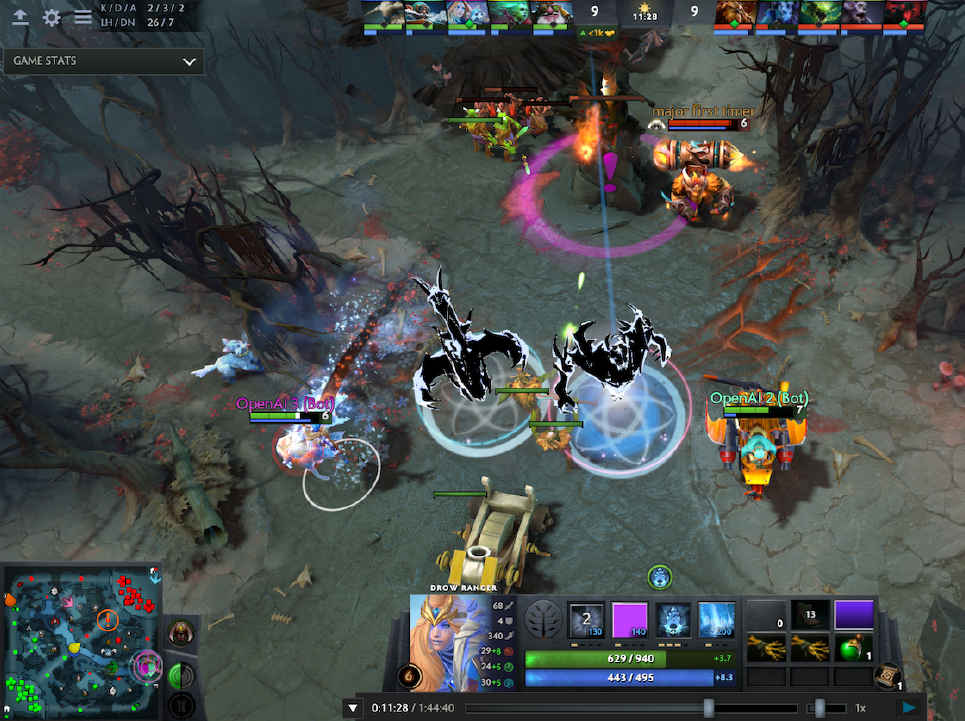
\includegraphics[width=\textwidth]{Figures/MADRL/openaifive.png}
        \caption{Multi-player video game}
        \label{fig:Dota2}
    \end{subfigure}
    \hfill
    \begin{subfigure}[c]{0.35\textwidth}
        \centering
        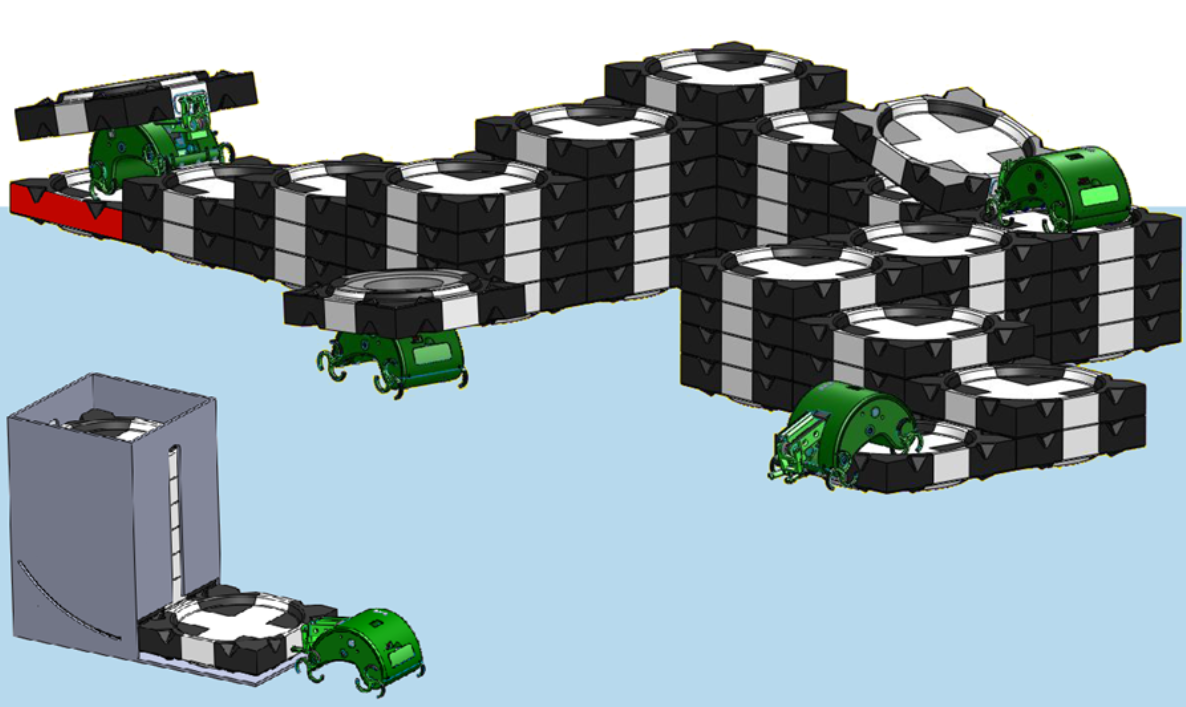
\includegraphics[width=\textwidth]{Figures/MADRL/termes.png}
        \caption{Multi-robot system}
        \label{fig:termes}
    \end{subfigure}
    \hfill
    \begin{subfigure}[c]{0.27\textwidth}
        \centering
        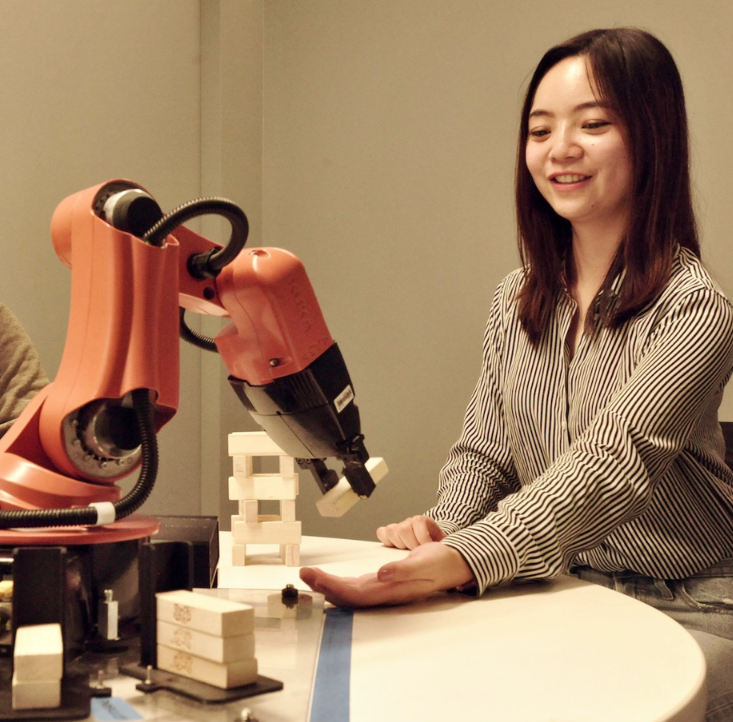
\includegraphics[width=\textwidth]{Figures/MADRL/hri.png}
        \caption{Human-robot interaction}
        \label{fig:hri}
    \end{subfigure}
    \caption{Types of multi-agent environments. (a) Social dilemmas, here the famous \textit{prisoners' dilemma}, extensively used in the game theory literature to devise multi-agent learning concepts and exact solutions. (b) Two-dimensional grid environments (here, level-based foraging;~\cite{Albrecht2013_Foraging}) that allow studying various multi-agent tasks in simplified settings. (c) Card and tabletop games (here, Hanabi;~\cite{Bard2020_Hanabi}) that often require learning complex strategies. (d) Multi-player video games (here, Dota 2, tackled by~\cite{OpenAI2019_DOTA2}) that offer rich environments demanding complex team-play. (e) Multi-robot systems (here, the TERMES construction robots;~\cite{Petersen2012_TERMES}), having to deal with high-dimensional robotic settings. (f) Human-robot interaction, with the need to build interfaces and adapt to human partners~\citep{Jung2020_TowerConstruct}.} 
    \label{fig:MAenvs}
\end{figure}


\section{Introduction}

% Why MAS and MAL
In most realistic environments, multiple entities interact with each other to fulfil an individual or a collective goal. With multiple entities, each with their personal reasoning, the outcome of one's actions also depends on the others' actions, thus increasing the difficulty of learning how to best behave. If entities are all capable of adapting and learning, then the environment becomes an ever-evolving sum of intersecting strategies. The problem of finding the optimal strategy becomes even more complex, as the best response to previously observed behaviours might not be true in future tries. The single-agent learning setting, used throughout Chapter~\ref{ChapterRL}, does not explicitly model these new problems and, thus, falls short in most of these cases. For this reason, the concept of multi-agent system (MAS) has been defined to better describe the dynamics of environments containing multiple intelligent entities, as found in human societies~\citep{Doran1995_EOS, Bousquet2004_MASEcosystem, Hamill2015_ABMEconomics}, games~\citep{Nowé2012_GameTheory, Owen2013_GameTheory}, or robotics~\citep{Parker2016_MRS, Rizk2019_CoopHeteroMRS} (see Figure~\ref{fig:MAenvs} for example of multi-agent environments). Multi-agent learning specifically tackles how learning takes place in MASs, how it can be harmed by having multiple agents, and how it can benefit from it. Multi-agent learning research comes from the intersection of many different views in software engineering~\citep{Ben-Ari2006_DistribProg}, distributed artificial intelligence~\citep{Stone2000_MASMachineLearning}, and game theory~\citep{Rosenschein1994_Encounter, LeytonBrown2008_GameTheory}; each one having proposed ways of modelling multi-agent interactions~\citep{Wooldridge2009_IntroMAS}. One possible way is to adapt and extend single-agent RL tools to fit the needs of MASs. Recent years have seen the development of multi-agent deep reinforcement learning (MADRL) algorithms, with a wide range of new approaches for tackling richer multi-agent environments. 

% What this chapter does
Many robotic applications involve interactions between multiple robots and/or humans~\citep{Parker2016_MRS}. In this context, MADRL is a potentially valuable tool for learning complex multi-agent behaviours in realistic environments~\citep{Orr2023_MADRLRobots}. But, to progress towards this objective, we need to ask ourselves: \textit{What does it mean to have robots operating in the real world? What should be the requirements when building intelligent robots and how should this impact the design of learning algorithms?} This thesis intends to provide answers to these questions by studying existing approaches and proposing new solutions for improving cooperative MADRL in the context of robotics. In this particular regard, we are faced with several observations about the related literature:
\begin{enumerate}
    \item Learning with multiple agents implies multiple theoretical and technical issues that are often treated separately or even ignored.
    \item Similarly, robotic domains establish several constraints and challenges that are not thoroughly investigated in MADRL research, despite a prevalent aspiration of applying these algorithms to robotic settings.
    \item The multi-agent (deep) reinforcement learning literature is extremely rich, with many orthogonal subjects of interest. This results in a domain that is hard to grasp and fully understand, with many works that are difficult to compare and evaluate.
\end{enumerate}
This chapter aims to propose a clarified view of the literature, providing insights and avenues for reflection on these three starting observations. In Section~\ref{sec:MALearning}, we start by formally defining important concepts and mathematical tools used in multi-agent RL. In Section~\ref{sec:MADRL_Context}, we introduce points (1) and (2), defining the challenges met in multi-agent learning and robotic settings, and looking at how they can overlap. 
To answer point (3), in Section~\ref{sec:MADRL_Review}, we present a short review of recent works in the MADRL literature. 
% Note that this is not a comprehensive review, but rather an overview of important research directions (see sec discuss for references to more complete reviews of related domains)
Finally, in Section~\ref{sec:MADRL_RobotPerspective}, we provide a personal reflection on the remaining shortfalls of MADRL research, specifically when dealing with robotic applications. We aim to highlight the major flaws of this line of work and identify potential areas of improvement.








% -------------------------------------------------------------------------------------------------

\section{Multi-Agent Learning: Definitions}\label{sec:MALearning}

% Multi-agent Learning
Multi-agent learning studies how learning can take place in environments where there are two or more intelligent agents. There is no theoretical limit to the number of agents in a MAS, but studies in this field are often limited to rather small groups of agents (say, from 2 to around 20), with larger groups being the subject of swarm robotics~\citep{Hamann2018_SwarmRobotics}. With a limited number of agents, multi-agent learning research can study more complex agent definitions and more intricate social dynamics. 

% Agents in MAS
Agents in a MAS are close to the RL agents defined in Section~\ref{sec:RL:Elements}. But, because they are now in a group, their definition may be completed accordingly. In addition to the three characteristics of \textit{reactiveness}, \textit{proactiveness}, and \textit{ability to learn}, defined in Section~\ref{sec:RL:Elements}, an intelligent agent is now also a \textbf{social} entity. This translates into having interactive abilities, which can be either \textit{explicit abilities}: e.g., communication (see Sections~\ref{sec:MAL:Comm_def} and~\ref{sec:MADRL:EmergentCommunication}), prediction of multi-agent outcomes (see Section~\ref{sec:MAL:Nash_Eq}), or agent modelling (see Section~\ref{sec:MADRL:AgentModelling}); or \textit{implicit abilities}: e.g., cooperation, coordination, attack/defence, negotiation, or bluffing. Taking this social aspect into consideration will influence the design of multi-agent learning algorithms. 




\subsection{Learning Framework: Dec-POMDP}\label{sec:MAL:Dec-POMDP}

% DecPOMDP
Because we want to study cooperation in robotic-like environments, we use the decentralized partially-observable Markov decision process (Dec-POMDP)~\citep{Oliehoek2016_DecPOMDP} as our learning framework. The Dec-POMDP is an extension of the MDP (as defined in Section~\ref{sec:RL:MDPs}) that allows the presence of multiple intelligent agents and models the fact that the environment is not fully observable: agents only observe a part of it through their sensors. Formally, it is defined as a tuple $\langle\mathbf{S},\mathbf{A},\mathcal{T},\mathbf{O},\mathcal{O},\mathcal{R},n,\gamma\rangle$ in which:
\begin{itemize}
    \item $n$ is the number of agents;
    \item $\mathbf{S}$ is the set of all possible states of the environment, often referred to as "global states" as they describe the environment entirely;
    \item $\mathbf{O}$ is the set of joint observations, with one joint observation $\mathbf{o}=\{o^1,...,o^n\}\in\mathbf{O}$ being a set of local observations (one for each agent);
    \item $\mathbf{A}$ is the set of joint actions, with one joint action $\mathbf{a}=\{a^1,...,a^n\}\in\mathbf{A}$ being a set of local actions (one for each agent);
    \item $\mathcal{T}$ is the transition function defining the probability $P(s'|s,\mathbf{a})$ to transition from state $s$ to next state $s'$ with the joint action $\mathbf{a}$;
    \item $\mathcal{O}$ is the observation function defining the probability $P(\mathbf{o}|\mathbf{a},s')$ to observe the joint observation $\mathbf{o}$ after taking joint action $\mathbf{a}$ and ending up in $s'$;
    \item $\mathcal{R}:\mathbf{S}\times\mathbf{A}\rightarrow\mathbb{R}$ is the reward function producing a single reward for all agents at each time steps;
    \item $\gamma\in[0,1)$ is the discount factor controlling the importance of immediate rewards against future gains.
\end{itemize}
Figure~\ref{fig:DecPOMDP} illustrates a time step in the Dec-POMDP framework. An important thing modelled in this framework is that agents may not have access to the global state of the environment $s_t$ (it is often even not defined). They only observe a sub-part of this global state through their sensors, which is represented by the local observations $o^i_t$. In a robotic environment, the local observation will be the result of the robot's sensors (e.g., camera, lidar, etc.). In simulation, the content of the observations is typically defined arbitrarily by deciding what an agent should be able to observe from the environment (e.g., its position, the relative positions of other agents, etc.). The joint observation $\mathbf{o}_t$, denoted in bold, is the concatenation of all local observations at step $t$ (and similarly for the joint action $\mathbf{a}_t$). 


\begin{figure}
    \centering
    \includesvg[width=0.7\linewidth]{Figures/MADRL/DecPOMDP.svg}
    \caption{Diagram illustrating the Dec-POMDP framework. At each step $t$, the environment is in a state $s_t$ that may be unknown by the agents. The joint observation $\mathbf{o}_t$ is produced by the environment, containing one local observation $o^i_t$ for each agent $i$. Each agent produces an action $a^i_t$, all actions being gathered in the joint action $\mathbf{a}_t$ that is to be executed in the environment. A single reward $r_t$ is produced and shared by all agents for evaluating step $t-1$. The red dotted line symbolises the multi-agent learning algorithm that can use the reward in various ways to train the agents.}
    \label{fig:DecPOMDP}
\end{figure}



\subsection{Multi-Agent Reinforcement Learning Tools}\label{sec:MAL:MARL_tools}

% Policy history and values
The Dec-POMDP framework allows the development of RL agents, with the basic RL tools adapted to take into consideration the multi-agent context. With multiple agents, the goal of the learning algorithm is to find the optimal \textbf{joint policy} $\pi=(\pi^1,...,\pi^n)$, with one \textbf{local policy} $\pi_i$ for each agent $i$, that maximises expected future returns. In the Dec-POMDP, local policies are conditioned on the action-observation history $h^i_t=(o^i_0,a^i_0,...,a^i_{t-1},o^i_t)\in \mathbf{H}=(\mathbf{O}\times\mathbf{A})^*$ that contains all previous local observations and actions in the current episode. Thus, we have one local policies $\pi^i(a^i|h^i):\mathbf{H}\times\mathbf{A}\rightarrow[0,1]$ for each agent. The \textbf{joint value functions}, related to the joint policy can be written as:
\begin{equation}
    V_\pi(\mathbf{h}_t)\coloneqq\mathbb{E}_\pi[G_t\ |\ \mathbf{h}_t]\text{ and }Q_\pi(\mathbf{h}_t,\mathbf{a}_t)\coloneqq\mathbb{E}_\pi[G_t\ |\ \mathbf{h}_t,\mathbf{a}_t]; \label{eq:JointValue}
\end{equation}
and similarly for the \textbf{local value functions} related to the local policy $\pi_i$:
\begin{equation}
    V_{\pi^i}(h^i_t)\coloneqq\mathbb{E}_{\pi^i}[G_t\ |\ h^i_t]\text{ and }Q_{\pi^i}(h^i_t,a^i_t)\coloneqq\mathbb{E}_{\pi^i}[G_t\ |\ h^i_t,a^i_t], \label{eq:LocalValue}
\end{equation}
with the discounted return $G_t$ defined as in RL (see Equation~\ref{eq:return}) and $\mathbf{h}_t=\{h^1_t,...,h^n_t\}$ the joint action-observation history. We will also denote the local policy of any agent $i$ as $\pi_{\theta_i}$, with $\theta_i$ the learnt parameters of agent $i$. Similarly, the joint policy can be written $\pi_\theta$, with the whole set of parameters $\theta=(\theta_1,...,\theta_n)$. 

% Actual use of history
We will see that MADRL algorithms usually do not explicitly use the action-observation history to condition the local policies. Some simply do not use it and condition only on the local observation. Others implement some kind of memory in the agent's policy (e.g., a recurrent neural network) to implicitly save some information about past steps in the agent's reasoning. 





\subsection{Communication}\label{sec:MAL:Comm_def}

% Intro communication
Multi-agent interactions may benefit from the ability to communicate information to other agents. Communicating efficiently requires knowing what information should be shared and how to share this information to be understood correctly. Learning these skills is a challenge in itself that has been thoroughly studied in dedicated lines of work~\citep{Austin1975_SpeechActs, Farrell1996_CheapTalk, Brighton2005_LanguageAsEvo, Galke2022_Emergent} and in the context of MADRL, as we will see in Section~\ref{sec:MADRL:EmergentCommunication} and more deeply in Chapter~\ref{ChapterComm}. In a MAS, communication can take multiple forms. Agents might develop implicit communication abilities, using physical actions to convey abstract information (e.g., pointing a finger towards an object). Agents might use a shared archive, similar to a blackboard in a room, to store information accessible to everyone. Or, they might be provided a collection of mechanisms for exchanging messages between agents. We focus on such explicit, message-based communication to describe how agents can learn to communicate. 

% Formal definition
Communication mechanisms can be defined in many different ways depending on when agents communicate, how they share information, and to whom they are allowed to communicate. Here, we define a formal framework for communication to describe its use in MADRL algorithms. Note that this framework might not fit all communication architectures perfectly, but it can be adapted if needed. 

We define communication as taking place during the action-selection process of the agents. After receiving their local observations, agents take part in a \textit{communication turn} where they can generate a message $m^i_t=f^i_{comm}(h^i_t,\theta_i)$ and send it to the other agents. We consider $f^i_{comm}$ as a learnt module of agent $i$, using a subset of $\theta_i$ (e.g., a dedicated neural network) to generate the message. The message can be sent to either all other agents, referred to as \textit{broadcasting}, or to a limited subset, e.g., within a certain range or choosing particular agents to target. Agents then receive incoming messages and use them according to their architecture. Some methods might allow repeating such communication turn multiple times to allow some form of discussion. Then, the incoming information is used to compute the generated action: $a^i_t\sim\pi_i(.|h^i_t,m_t)$, where $m_t$ refers to the incoming messages. 



\subsection{Nash Equilibrium}\label{sec:MAL:Nash_Eq}

% Definition
An important concept from game theory is the Nash equilibrium, introduced by~\cite{Nash1950}. It represents a stable joint policy state where no player can gain an advantage by changing their individual strategy, provided that the other players' strategies remain unchanged. This equilibrium can take various forms. A deterministic Nash equilibrium requires agents to always choose a particular joint action. A stochastic Nash equilibrium is one describing a stochastic joint policy, where agents select their actions given a specific equilibrium distribution. Nash equilibria are pivotal in multi-agent systems research, as they help predict the behaviour of agents interacting in competitive or cooperative environments. 

% Equilibrium selection
Importantly, there may be multiple Nash equilibria in a particular environment, with some equilibria yielding better returns than others. Thus, a problem of equilibrium selection arises to avoid suboptimal equilibria and efficiently converge to the optimal one~\citep{Harsanyi1988_EqSec, Kalai1993_Rational, Bowling2002_WoLFIGA, Conitzer2007_Awesome}. 
While equilibria are instructive for understanding valuable long-term strategies, their direct application may be flawed in dynamic and unpredictable environments~\citep{Shoham2007_MAL}. Additionally, they are impractical, if not impossible to compute in high-dimensional and non-simulated environments, as they require knowing the outcomes of all actions in all possible states. Nonetheless, Nash equilibria remain a significant concept in multi-agent learning, helpful for illustrating the dynamics of some multi-agent scenarios.









% -------------------------------------------------------------------------------------------------

\section{Context: Challenges in Multi-Agents Robotic Domains}\label{sec:MADRL_Context}

% Intro
Working towards learning behavioural strategies for multi-robot systems requires first understanding the implications of learning in such environments. The multiplicity of intelligent agents in an environment has many important impacts on how these agents are able to learn, disrupting basic RL techniques and imposing strong architectural choices. Similarly, learning in robotics faces several obstacles that hinder the applicability of algorithms designed to learn in games and simulations~\citep{Pierson2017_DRLinRobots}. In this section, we define the challenges of both domains, look at how they intersect, mention some basic or foundational approaches to tackle them, and discuss their impact on the design of learning algorithms. 



\subsection{Learning with Multiple Agents}\label{sec:MAL_issues}

\subsubsection{Non-Stationarity}\label{sec:MAS:NonStation}

% Non-stationarity
The problem of non-stationarity refers to the continuously changing nature of the learning environment. It occurs in single-agent RL, as training the agent changes its behaviour, thus modifying the nature of its future interactions with the environment. But, in the multi-agent setting, non-stationarity is greatly amplified by having all agents change their behaviour after each training phase. 
From the point of view of an agent, the optimisation problem (i.e., "finding the best policy to maximise future returns") changes after each training phase, because the distribution of states and the outcome of actions change. 
This leads to a moving target problem, where continuous co-adaptation can induce unstable training. 
This is especially bad for RL algorithms, as they bootstrap the learnt estimates to determine the best solution to the optimisation problem. If this problem changes too much after each training phase, the learnt estimates can end up ineffective. 
In addition, the optimisation problem being constantly evolving, past experiences are made irrelevant for future training phases as they depict obsolete interactions. This makes the use of experience replay unusable without specific adaptation~\citep{Foerster2016_SolveRiddles}. 

% Pistes pour résoudre le problème
Non-stationarity is a major issue preventing single-agent RL algorithms from working in multi-agent settings. To tackle this problem, multiple approaches have been proposed. In Section~\ref{sec:MADRL_Review}, we will see that using centralised information during training can help constrain the effects of non-stationarity. Because experience replay is such an important part of making DRL function well, some works have proposed solutions to adapt it for MADRL by ensuring that all agents train on concurrent time steps~\citep{Omidshafiei2017_DecentrMultiTask} and giving less weight to older experiences in the replay memory~\citep{Foerster2017_StabExpReplay}. While the concurrent replay method has been widely adopted, this does not completely solve the issue. Replay memories in MADRL are often set to discard old experiences earlier than in single-agent RL to prevent learning from too irrelevant data.



\subsubsection{Credit Assignment}\label{sec:MAL:CreditAssign}

% Credit assignment problem
Credit assignment refers to the problem of finding how each past action contributed to the obtained rewards. As for non-stationarity, this problem exists in single-agent RL, with actions contributing to rewards obtained in the future, requiring a form of \textit{temporal credit assignment}. 
But this becomes harder with multiple agents as, at each step, multiple actions are performed simultaneously by different agents. Knowing the marginal contribution of each action is a crucial requirement for evaluating each local policy accordingly. 
This \textbf{multi-agent credit assignment} problem can be examined from the point of view of the whole MAS, looking at \textit{"how much each agent contributed to the obtained return?"}, or from the point of view of a single agent, answering the question \textit{"was my success (or failure) due to my actions, or to some other agent's actions?"}. 
This problem is particularly difficult in the Dec-POMDP framework where all agents share a common reward signal. In such cases, a "lazy" agent could be reinforced into doing nothing because the other agents manage to solve the task on their own. However, it is worth noting that the problem persists if each agent gets its own individual reward (and, similarly, in competitive settings), because a local reward might have been caused by another agent's actions. 

% Exact solutions and counterfactual utilities
To tackle the multi-agent credit assignment problem, some methods have been developed for trying to model the marginal contributions of each agent. Exact solutions exist in simple, controlled environments, like the \textit{Shapley value}~\citep{Shapley1953} that evaluates an agent with the expected gain in utility of having this agent contribute in any possible coalition of agents. But this value is computationally very expensive and even approximations are hardly applicable to environments outside the game-theoretic framework or with a large number of agents~\citep{Fatima2008_ShapleyLinApprox, Michalak2014_ShapleyEffComp, Wang2020_ShapleyQValue, Wang2022_SHAQ}. 
Another approach is to compute the marginal contribution of each action as the difference between the observed outcome and a counterfactual outcome where the evaluated action was not performed. The \textit{wonderful life utility} (WLU;~\cite{Wolpert1999_WLU}) replaces the action by a "null" action and simulates the presumed return: $WLU(a_i)=G(\mathbf{a})-G(\mathbf{a}_{-i},a_i=\text{null})$, with $G$ the evaluation function and $\mathbf{a}_{-i}$ the joint action without action $a_i$. The \textit{aristocrat utility} (AU;~\cite{Wolpert2002_AristoUtility}) takes as counterfactual metric the expected outcome from the truncated joint action: $AU(a_i)=G(\mathbf{a})-\mathbb{E}(G|\mathbf{a}_{-i},s)$, with $s$ being the state in which action $a_i$ was performed. However, these utilities are impractical to compute in high-dimensional, stochastic environments. In Sections~\ref{sec:MADRL:CentralCritic} and~\ref{sec:MADRL:ValueFac}, we will introduce recent approaches, based on MADRL, to the credit assignment problem that better fit more realistic settings. 


\subsubsection{Coordination}\label{sec:MAL:Coordination}

% Definition of coordination
In many cooperative multi-agent tasks, agents are required to coordinate their actions to fulfil the objective. Robots might have to lift a heavy object together. In games played in teams, coordination between teammates is often crucial to successful tactics~\citep{Samvelyan2019_SMAC, Bard2020_Hanabi}. Thus, coordination is often a pursued ability in cooperative multi-agent learning. Coordination can be defined, in the multi-agent context, as the ability of an agent to synchronise its local actions with the anticipated behaviour of other agents to achieve a particular objective. This ability encompasses a wide set of knowledge the agents must acquire: knowledge about the environment dynamics, about how the task is completed, and about the other agents' strategies. Learning all this can be extremely complicated, especially in partially observable environments where local information is often insufficient to understand the full state of the environment. 

Coordination skills may be learnt with different approaches. First, by acquiring a thorough knowledge of the joint policy search space to know how to behave in any situations. This can be related to a problem of multi-agent exploration of the joint policy space, which we study more deeply in Chapter~\ref{ChapterJIM}.
Another approach would be to have an explicit mechanism for coordinating actions during execution. This can be tackled in various ways. In Section~\ref{sec:MADRL:AgentModelling}, we review methods that enable agents to learn a model of the other agents' policies, allowing them to coordinate their choice. Communication can be a handy mechanism for exchanging local information and reaching a consensus on the best way to act (see Section~\ref{sec:MADRL:EmergentCommunication} and Chapter~\ref{ChapterComm}). Finally, coordination graphs~\citep{Guestrin2002_CoordGraphs, Bohmer2020_DeepCoordGraphs, Li2021_DeepImpCoordGraphs} more explicitly model coordination by learning pairwise joint value functions. 



\subsubsection{Scaling}\label{sec:MAL:Scaling}

A major issue of all multi-agent learning algorithms is how they deal with scaling to larger state and action spaces and, especially in the case of MASs, to a larger number of agents in the system. Being able to handle more agents efficiently makes an algorithm more applicable to various settings. But, this is not elementary, as scaling exacerbates all issues faced by multi-agent learning. Non-stationarity is increased because having more agents in the system means the environment changes more after each training step. Credit assignment is harder because the outcomes depend on more local actions. Learning value and policy functions is more difficult, as they depend on more independent elements and, thus, the search space is larger. On a more technical note, having more agents makes training more computationally expensive. As in RL, the use of deep learning techniques can help for dealing with scaling. It helps generalising to unseen configurations of the environment, partly compensating for the larger search spaces. In Section~\ref{sec:MADRL:IL}, we will see that having agents learn independently can help with scaling, but it also implies some important downsides. 




\subsection{Learning in Robotic Domains}

\subsubsection{Domain Complexity}\label{sec:MAL:DomainComplexity}

Going towards learning in robotic environments, an important obstacle to successful learning is the complexity of realistic environments. Many multi-agent environments simplify the definition of states and actions substantially to focus on particular multi-agent dynamics (e.g., two-dimensional grid level-based foraging, as shown in Figure~\ref{fig:lbf1}, to study how coordination can arise). But, to apply learning algorithms to robotic domains, they must be capable of handling the full complexity of realistic state and action definitions. This complexity takes three different forms: high-dimensionality, continuity, and multi-modality. 

\textbf{High-dimensional} states and actions are made of many components that each carry some information. Take, for example, a robotic hand manipulating objects. For observing its environment, it might use an RGB (red-green-blue) camera producing images made of thousands of three-valued pixels (one value for each colour). Understanding each image requires knowing how these numerous values relate with each other to compose high-level information. For manipulating objects, the robotic hand must control a large number of motors at once to achieve the desired motion. Each motor necessitates its own policy, but all policies must coordinate to achieve the desired behaviour. Note that, such high-dimensional action space can benefit from being formulated as a multi-agent problem, with each joint being handled by one agent~\citep{Sartoretti2019_DistribArticulat}. 

Robots usually deal with \textbf{continuous} inputs and outputs. For example, pixel values can be represented as a continuous value of colour intensity. Continuous angles of rotation are used to precisely articulate joints. Having continuous states and actions implies that the respective search spaces are infinite. This requires the ability to generalise well to handle previously unseen states: in a continuous state space, a robot will never experience the same state twice so it needs to use its experience in very similar states to know how to react. Handling continuous states and actions also requires specific techniques. In Chapter~\ref{ChapterRL}, we have seen how tabular methods are unable to handle continuous state and action spaces, as they require learning estimates for each possible state-action pair (see Section~\ref{sec:RL:Qlearning}). Similarly, deep Q-learning is limited to discrete action spaces as it learns the values of a discrete set of pre-defined actions. Thus, dealing with continuous spaces imposes strong design constraints. 

Finally, robots often encounter \textbf{multi-modal} states and actions, which are composed of multiple different types of information. In addition to the RGB camera, the robotic hand might have tactile sensors on each finger that generate precise haptic information on how the object is being grasped. Actions may also be distributed on different types of actuators: e.g., wheels to navigate in a room, hands to grasp objects, and voice to communicate. Multi-modality requires the controller to understand different types of information and recognise their relationships and interactions. 

These input and output complexities each require specific care and altogether make learning more difficult. Deep learning techniques are an important tool for dealing with this level of complexity. They allow automatic learning of high-level representations from high-dimensional data~\citep{Simonyan2015_VGG}, generalisation in continuous spaces~\citep{Schulman2016_GAE}, and fusing of multi-modal data~\citep{Radford2021_CLIP, Driess2023_PaLME}. With the right learning approach and enough resources, deep learning enables efficient learning of complex robotic behaviour~\citep{Pinto2016_SelfSupervisedGrasp, OpenAI2020_DextHandManip}. However, using deep learning has some notable drawbacks such as sample inefficiency and computational cost. When used in the context of RL, deep learning techniques are useful to open the range of potential applications, but RL techniques still require extensive work to suit robotic domains well~\citep{Sunderhauf2018_Limits, Ibarz2021_Howto}. 


\subsubsection{Partial Observability}\label{sec:MAL:PartialObs}

All realistic robotic environments are inherently partially observable. It is practically impossible to capture the full complexity of a real-world setting within a single state vector. A robot typically accesses information about its environment by observing it with its own sensors, providing it with a subjective view of its immediate surroundings. This limited perspective does not offer a complete description of the full state of the environment. To achieve its objective, a robot must infer some information based on its past experiences and observations from previous steps. 

In the context of multi-agent RL, the Dec-POMDP, defined in Section~\ref{sec:MAL:Dec-POMDP}, is useful for modelling this environmental uncertainty. Similar to realistic robotic settings, agents within a Dec-POMDP only observe a subjective subset of the complete state of the environment. The resulting uncertainty significantly increases the difficulty of learning optimal policies. To overcome this, robots require specific tools. In single-agent POMDPs, agents can learn to infer the current state of the environment from their incomplete observations~\citep{Abbeel2006_Helicopter, Lee2019_SLAC}. However, in a multi-agent setting, this is significantly harder as the state also depends on the actions of other agents~\citep{Papadimitriou1987_Complexity, Oliehoek2016_DecPOMDP}. Memory can be a valuable tool in dealing with uncertainty, enabling agents to remember previous observations during an episode to better infer the current state~\citep{Hausknecht2015_DRQN}. Communication can also play a crucial role, allowing agents to share their individual subjective knowledge, thus cooperating to build a more accurate representation of the current state (see Section~\ref{sec:MADRL:EmergentCommunication} and Chapter~\ref{ChapterComm} for more detail). 


\subsubsection{Reality Gap}\label{sec:MAL:RealityGap}

Because RL requires thousands of experiences to converge to an efficient strategy, a promising approach to learning robotic tasks is to train in simulation and then apply the learnt policy on the real robots. However, this transfer is challenging due to numerous subtle differences between the simulated environment and the real world, a problem known as the \textbf{reality gap}~\citep{Jakobi1995_RealityGap}. Even the most sophisticated simulations fall short of accurately reproducing real-world dynamics. Real robotic sensors and actuators have imperfections that are often not modelled in simulations. These minor discrepancies accumulate, causing a policy that performs well in simulation to fail when deployed on a real robot. To leverage extensive training in simulation, techniques must be developed to enable efficient simulation-to-reality (sim-to-real) transfer~\citep{Ju2022_Sim2Real}. 

One possible sim-to-real approach is to develop models that adapt quickly and effectively to new domains~\citep{Rusu2017_ProgressiveNets}. This can be facilitated by learning the critical characteristics shared between the training and execution domains~\citep{Gupta2017_InvariantFeatureSpace, James2019_Sim2Real}. Another strategy, which can complement the first, is domain randomisation. This technique involves slightly randomising observations and actions during training in simulation, making RL agents more robust to minor discrepancies in their inputs and outputs~\citep{Tobin2017_RealityGap, Chebotar2019_Sim2Real, OpenAI2020_DextHandManip}. Lastly, hierarchical learning offers a promising approach to developing transferable policies~\citep{Nachum2020_HierchicalSim2Real, DAmbrosio2024_PingPong}. Assuming that the reality gap affects lower-level actions more, it should be easier to learn a transferable high-level policy that selects macro-actions (e.g., find an apple)~\citep{Amato2019_MacroActions}. Low-level policies for executing these macro-actions with basic actions (e.g., move forward) can be learnt more easily within the target domain. 



\subsubsection{Embodiment}\label{sec:MAL:Embodiment}

Contrary to most computer programs, the controller of a robot is \textbf{embodied}: it is situated within a concrete body that lives inside an environment~\citep{Pfeifer2006_Embodiment}. There are many different views of embodiment from philosophy, psychology, cognitive science, and artificial intelligence, describing the role of embodiment in learning and intelligence~\citep{Lakoff1999_PhiloInTheFlesh, Barsalou2003_SocialEmbodiment, Kiverstein2012_Embodiment, Sunderhauf2018_Limits}. Here, we define some useful notions for appreciating the various implications of control and learning in robotics.
\textbf{Physical} embodiment relates to the instantiation of the controller in a physical body that can sense and act upon its environment. 
\textbf{Temporal} embodiment refers to the fact that robots experience their environment through sequences of strongly correlated states. This has important implications for the treatment of both past states, on which the present state depends, and future states, which can be influenced by the robot's actions. 
What we call \textbf{composite} embodiment refers to the composite nature of a robot, made of many interconnected parts that all serve a specific purpose in the life of the robot. \cite{Ziemke2003_Embodiment} calls this "organismoid" to relate the composite body of robots to that of a living organism in which the presence of organs may play a major role in the development of commonsense intelligence~\citep{Lakoff1999_PhiloInTheFlesh}. 
Finally, \textbf{social} embodiment describes the fundamental relation between intelligent entities in the environment, and how these social relations may shape intelligence~\citep{Barsalou2003_SocialEmbodiment}. In the context of robotics, other entities may be other (potentially heterogeneous) robots, humans, or even animals. Such interactions are extremely diverse and may be dictated by implicit or explicit social rules. 
All these notions manifest in robotics, but not necessarily in other domains of computer science and artificial intelligence. Thus, it is instructive to consider these notions to build better robotic systems.

Embodiment is not a problem in itself but an essential perspective for understanding the challenges of robotic applications. Being embodied in all the forms described above has many important implications. 
The physical and temporal views of embodiment, put together, imply a capacity to interact with the environment: the robot needs to perform actions to gather information and alter the environment. This introduces safety concerns, as actions in a physical environment may result in catastrophic outcomes. It also implies a highly dynamic range of environmental situations: in the real world, the people, objects, and furniture present in the room might change over time; a single type of object can be associated with many different forms and colours; and one task can be performed in different environmental settings (e.g., different ground textures or weather conditions) which may change during the robot's life. 
The robot's composite form entails the need to account for the inherent characteristics of its robotic parts: a particular sensor might require a specific behaviour to gather information properly, or any sensor or actuator may have flaws or momentarily malfunction. 
Finally, social embodiment implies the need to study the dynamics of interaction between multiple robots, as in MAS research, and between robots and humans (see Section~\ref{sec:MADRL:Interaction}). 
%Human-robot interaction (HRI) is a long-standing problem in robotics~\cite{Bartneck2020_HRI}. While some works focus on studying HRI, we argue that it would be valuable to more generally think of robots as entities living in human-populated environments. 

It is important to note that, while physicality is an important aspect of embodiment, simulations are still a useful tool for studying embodiment. Simulated environments accurately replicate many challenges linked with embodiment: interaction with the environment, temporal embodiment, and social interactions. However, some other aspects are harder to emulate: accurate physical dynamics, variety and dynamicity of the environment, malfunctions, and human-robot interactions. Thus, simulations are still relevant for addressing learning in robotics, but their shortages should not be overlooked and, if possible, addressed accordingly with real-world experiments. 


\conclusionseparator

\noindent
Challenges in multi-agent learning and robotics are numerous and, when combined, often exacerbate each other, making multi-robot environments particularly challenging. Due to this great multiplicity of issues, it is common for some problems to be addressed separately. However, this leads to the domain of multi-agent learning research being highly fragmented, with many concurrent lines of work that are difficult to compare. To advance towards the learning of complex behaviours in multi-robot environments, multi-agent learning needs to integrate the inherent challenges of robotics and develop methods that efficiently tackle all issues of multi-agent learning. In the next two sections, we will review the main directions of multi-agent reinforcement learning research and then reflect on how they address the specific problems of robotics. 










% -------------------------------------------------------------------------------------------------

\section{Methods in Multi-Agent (Deep) Reinforcement Learning}\label{sec:MADRL_Review}

To tackle multi-agent environments, RL algorithms have been adapted and extended in various ways. As with single-agent RL, deep learning has enabled addressing more complex multi-agent environments. In this section, we present a survey of state-of-the-art MADRL algorithms. We focus on some important techniques employed in the past few years to produce efficient algorithms. Our objective is to present the different approaches and explain the functioning of state-of-the-art algorithms that are frequently found in the literature and which we may use in subsequent chapters of this thesis.


% main avenues of MADRL -> core methods that may be used as basis for building more specific approaches
% 


\subsection{Multi-Agent Learning Paradigms}\label{sec:MAL:Paradigms}

% Intro learning paradigms
Designing a multi-agent learning algorithm requires first choosing how we consider one agent in relation to the MAS. This choice will dictate how information can be used for training the agent's policy and for executing it. In MASs, the gathering of information about the environment is always done locally by each agent, through the local observations $o_t^i$ (see Figure \ref{fig:DecPOMDP}). The processing of this information, however, can be done in various ways depending on our assumptions of how information can flow in the MAS. These assumptions will greatly impact the design of the resulting algorithms, as they dictate what information is available to them during training or execution. Here, we examine how, what, and when information can or should be centralised. By centralising information, we mean that the algorithm gathers the local observations together (i.e., it has access to the joint observation) and uses them during either the training phase to improve the learning update, the execution phase to improve local policies, or both. Note that this does not include communication, as defined in Section~\ref{sec:MAL:Comm_def}, that involves the agents actively choosing what information they should share with others. Centralising some information can greatly improve the efficiency of multi-agent learning algorithms. But, centralisation, if it is even possible, comes at several costs in terms of algorithmic conception and complexity. Thus, different MA(D)RL algorithms may prefer different levels of centralisation depending on environmental constraints and design decisions. They can be classified into three main categories that define how information is allowed to flow in the MAS during training and execution.

% Centralised Training and Execution
The \textbf{centralised training and execution} (CTE) paradigm allows information to be shared between agents at all times. This means that the agents' policies might be conditioned on information coming from other agents. 
Centralising information can take many different forms: sharing other agents' observations, internal hidden states, learnt parameters, generated value estimates, or policy outputs. This allows agents to generate better predictions and to have more information at hand during training to stabilise training. For example, a local policy conditioned on the joint observation, $a_{i,t}\sim\pi_i(.|\mathbf{o}_t)$, will have more information about the environment, allowing better prediction of the best action to choose. A more extreme version of this would have a single controller centralising all local observations and generating the joint action: $\mathbf{a}_t\sim\pi_{central}(.|\mathbf{o}_t)$. This would reduce the problem to a single-agent one, preventing the issues of multi-agent non-stationarity and credit assignment. 
But, these methods imply that the search spaces (for learnt estimates) grow exponentially with the number of agents, making such solutions poorly scalable. 
Additionally, in many environments, it might not even be possible to share information between agents. In realistic scenarios, agents are often independent and might not be connected to a central unit that can centralise and redistribute information freely.

% Decentralised training and execution
At the opposite side of the spectrum, \textbf{decentralised training and execution} (DTE) considers that no information can ever be centralised. 
This is a far more realistic assumption as it does not rely on an algorithmic-level connection required to pass information between agents. 
It is also more computationally efficient to learn estimates in tighter observation and action spaces. So it allows better scaling to a large number of agents. 
However, because less information is at their disposal to train and compute estimation functions, these algorithms can learn less efficiently and suffer more from non-stationarity. 
Note, again, that this does not forbid having communication between agents. In fact, decentralised agents would largely benefit from learning an efficient way to discuss with partners to share local information and coordinate their actions~\citep{Cao2018_Negotiation}.

% CTDE
To improve on DTE without losing the decentralised execution, a middle ground can be found with \textbf{centralised training and decentralised execution} (CTDE). In CTDE, information is allowed to be shared during training, but agents are kept totally independent during execution. Because training is usually done in a controlled environment, we can often make the reasonable assumption of being able to centralise some information during training. 
This allows a range of simplifications, with varying degrees of assumptions on how information can be centralised: from ensuring agents are trained on concurrent steps~\citep{Omidshafiei2017_DecentrMultiTask}, to learning centralised value functions (see Section \ref{sec:MADRL:CentralCritic}). In general, sharing some information makes RL training easier by reducing non-stationarity and compensating for partial observability. To ensure that execution is decentralised, the agents' policies are required to be conditioned only on local information, i.e., $a_i\sim pi_i(.|o_i)$. Because decentralised execution is such an important requirement and centralising information during training allows great improvements in RL training, the CTDE paradigm is the most preferred one today for MADRL algorithms.

% REFS A220



\subsection{Independent Learning}\label{sec:MADRL:IL}

A seemingly simplistic approach to the multi-agent problem is to consider each agent totally independently of the rest of the MAS, ignoring other agents, as if they were parts of the environment. This is often referred to as Independent Learning (IL; \cite{Tan1993, Claus1998_CoopMARL, Tampuu2017_IDQN}), where each agent can be trained independently with single-agent RL methods. 
But, a fully decentralised version of IL suffers badly from non-stationarity as the environment, composed of other learning agents, is continuously changing~\citep{Tan1993, Foerster2016_SolveRiddles}. 
\cite{Jiang2022_I2Q} solve the problem of non-stationarity by learning from a surrogate transition probability that considers other agents will act optimally. But this requires strong assumptions on the environment, especially that it is deterministic.
Thus, some assumptions from CTDE might be adopted to facilitate IL. For example, IL agents often share the parameters of their learnt policy or value functions \citep{Tan1993, Foerster2016_SolveRiddles, Gupta2017_PSTRPO, SchroederDeWitt2020_IPPO}, allowing faster convergence. To maintain diverse behaviours, the policies are conditioned on a unique identification number corresponding to the agent. To enable the use of experience replay in a decentralised algorithm, \cite{Omidshafiei2017_DecentrMultiTask} introduced concurrent experience replay for training agents on the same environment steps during each update. This ensures that independent learners have a common training schedule, thus mitigating the effects of non-stationarity. 
While IL seems simplistic, it has actually been shown to be competitive with more centralised alternatives~\citep{SchroederDeWitt2020_IPPO, Lyu2021_DecentralisedCritic, Jiang2024_DecentralizedMARL}.
This simplicity allows a great deal of freedom when designing training procedures. The self-sufficiency of agents makes it possible to modify the teams at will. For example, \citet{Jaderberg2018_FTW} trains a large population of independent agents, changing the team regularly so they learn to be robust to different partners and opponents. 

% REFS A223, Tan1993

\subsection{Multi-Agent Actor-Critics}\label{sec:MADRL:CentralCritic}

The CTDE framework requires only that the local policies are decentralised, that is, they must be conditioned on local information only (i.e., observations or history). Centralised information may be used, however, to improve the learning of these local policies. Therefore, a natural implementation of this paradigm is to use the actor-critic framework with decentralised actors and a centralised critic. Because the critic is used only to train the actor (see Section \ref{sec:Policy:Actor-Critic}), we can use centralised information to improve the value estimates learnt during training. The \textbf{multi-agent DDPG} (MADDPG; \cite{Lowe2017_MADDPG}) introduced this approach by having one DDPG-based actor-critic (see Section~\ref{sec:DRL:DDPG}) for each agent, but allowing the critics to use the joint observation to compute the local action-value estimates (see Figure~\ref{fig:MADDPG}). By using the information collected by all agents instead of only the local observation, the critic has more information on the current state of the environment to better estimate the action-value function. This also decreases the effects of non-stationarity: because the critic knows the state of other agents, it is less sensitive to changes in other agents' policies. 

This centralised critic idea has been widely used for its intuitive advantages. It has been extended to include memory with a recurrent neural network used in both the decentralised policies and the centralised critic~\citep{Wang2020_RMADDPG}. Other actor-critic algorithms have been implemented this way, with multi-agent PPO (MAPPO;~\cite{Yu2021_MAPPO}), multi-agent TD3 (MATD3;~\cite{Ackermann2019_MATD3}) and multi-agent SAC (MASAC;~\cite{Yu2021_Benchmark}). \citet{Iqbal2019_MAAC} added an attention mechanism in the centralised critic to better combine the centralised information. Finally, \citet{Foerster2018_COMA} used a centralised critic to improve credit assignment with their counterfactual multi-agent policy gradient (COMA). Having a centralised critic allows them to efficiently compute a marginal contribution for each local action, by computing the advantage of taking the action compared to all other possible actions: $A^i(\mathbf{h},\mathbf{a})=Q(\mathbf{h},\mathbf{a})-\sum_{a^{i\prime}}\pi^i(a^{i\prime}|h^i)Q(\mathbf{h},(\mathbf{a}^{-i},a^{i\prime}))$.

The nature of the centralised information used as input to the critic can vary. The joint observation is used often~\citep{Lowe2017_MADDPG, Iqbal2019_MAAC}. Memory-equipped agents can extend this with the joint history~\citep{Foerster2018_COMA, Wang2020_RMADDPG, Yu2021_MAPPO}. But, it has also been proposed to use the global state of the environment $s_t$, if it is defined and accessible~\citep{Lowe2017_MADDPG, Foerster2018_COMA}. This is often described as preferable because the global state would be a more condensed and complete description of the environment compared to the joint observation. However, it has been shown that using the global state can result in a higher variance in training as a result of introducing bias~\citep{Lyu2023_CentralisedCritics}. Additionally, defining the global state is a problem on its own, which might not be straightforward in some environments. In fact, in rich and complex settings (e.g., the real world), it might be impossible to describe the state fully. Thus, choosing a particular state definition is a complex design choice that can have important impacts on training. 

% MADDPG
\begin{figure}
    \centering
    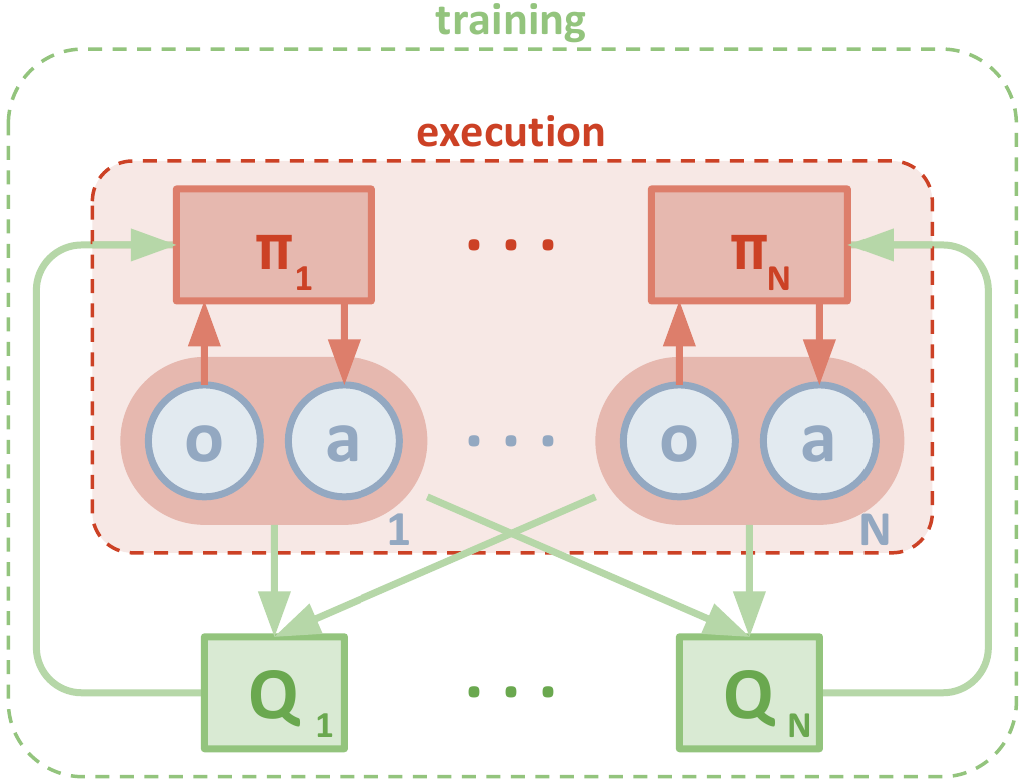
\includegraphics[width=0.48\linewidth]{Figures/MADRL/maddpg.png}
    \caption{The MADDPG architecture~\citep{Lowe2017_MADDPG} illustrating the centralised critics training decentralised policies. Each agent has a local policy used during training and execution, and a centralised critic, conditioned on the joint observation, used only during training.}
    \label{fig:MADDPG}
\end{figure}




\subsection{Value Factorisation}\label{sec:MADRL:ValueFac}

% Value factorisation concept
In Section~\ref{sec:MAL:CreditAssign}, we presented the multi-agent credit assignment problem that arises when multiple agents share a common reward signal and need a way to measure the contribution of their behaviour towards the observed common outcome. 
In such settings with a common reward signal, learning the value of local action $a^i$, with respect to the global return $G$ (as in Equation~\ref{eq:LocalValue}), can be problematic because $G$ does not depend only on $a^i$, but also on the other agents' actions. 
In Section~\ref{sec:MAL:CreditAssign}, we introduced methods that tackled this issue by computing a marginal contribution of each action. But, defining an effective marginal contribution can be tricky and computing it is usually expensive. 
Instead, another approach would be to learn the action-values of each action with respect to their real, unknown contribution, knowing that they are related in some way to the known common return. In other words, given the joint action-value $Q(\mathbf{h},\mathbf{a})$ estimating the expected global return (see Equation~\ref{eq:JointValue}) and local action-values $Q^i(h^i,a^i)\coloneqq\mathbb{E}_{\pi^i}[u^i\ |\ h^i,a^i]$, with $u^i$ the \textit{local utility} measuring the contribution of agent $i$ in $G$, we need to find how the local values compose the joint value:
\begin{equation}
    Q(\mathbf{h},\mathbf{a})=f(\{Q^i(h^i,a^i)\}_{1\leq i\leq n},\mathbf{h}).
\end{equation}
The function $f$ describes how each local value contributes to the joint value, depending on the joint history. Given the global return $G$, \textbf{value factorisation} (or "value decomposition") approaches learn the joint action-value and a way to decompose it into local action-values (i.e., function $f$). Value factorisation is a form of implicit credit assignment where we learn local value functions by learning how they compose the global value. 

% IGM property
Learning this properly allows having local action-value functions that can be used for choosing greedy local actions for each agent. Because the objective is to maximise the global return, this requires that greedy local actions lead to optimal joint actions. This has been referred to as the \textbf{individual-global-max} (IGM; \cite{Rashid2018_QMIX}) property, requiring that choosing the greedy joint action with respect to the joint action-value corresponds to choosing greedy local actions with respect to each local action-value, i.e.:
\begin{equation}
    \argmax_\mathbf{a}Q(\mathbf{h},\mathbf{a})=\{\argmax_{a^i}Q^i(h^i,a^i)\}_{1\leq i\leq n}. \label{eq:IGM}
\end{equation}
Respecting this property is essential to be able to use the learnt local action-values for local action selection. Thus, a multi-agent value-based learning algorithm that follows the IGM principle can fit into the CTDE paradigm, with decentralised local action-values used during execution, trained in a centralised manner with the help of a learnt joint action-value. 

% VDN
\cite{Sunehag2018_VDN} introduced this idea with their \textbf{value decomposition network} (VDN), making the simple assumption that local action-values should sum up to the joint action-value:
\begin{equation}
    Q(\mathbf{h},\mathbf{a})\approx\sum_{i=1}^nQ^i(h^i,a^i).\label{eq:VDN}
\end{equation}
With this assumption, $Q$ is differentiable with regard to each $Q^i$. Thus, VDN is able to learn individual action-values, parameterised as deep neural networks, from the DQN objective (see Equation~\ref{eq:DQN}) completely end-to-end. This linear version of value factorisation has the advantage of simplicity and being computationally lightweight, which allows excellent scalability. 

% QMIX
While this linear decomposition is intuitively logical and follows the IGM property, there is no guarantee that the true factorisation function $f$ is a linear transformation of local utilities. Therefore, the formulation of VDN limits the factorisation operation and the learnt representations of joint and local action-values. To address this, \textbf{QMIX}~\citep{Rashid2018_QMIX} introduces a separate "mixing" neural network that takes the local action-values and the global state as input, and outputs the joint action-value: $Q(s,\mathbf{a})=f_{MIX}(\{Q^i(h^i,a^i)\}_{1\leq i\leq n},s)$ (see Figure~\ref{fig:QMIX}). Note that, in their implementation, they consider that the global state $s$ is available, but it can be replaced by the joint observation of history if needed. The mixing network learns a factorisation function that depends on the current state of the environment, allowing much richer factorisation capacities. To ensure that the IGM is respected, the mixing of local values must be monotonic: if a local value increases, the joint value must increase too, i.e., $\frac{\partial f_{MIX}}{\partial Q^i}\geq 0$. This monotonic constraint is ensured by having the weights of the mixing network be positive. But, this constraint must be applied only for the local action-values, not for the state. To allow this, QMIX employs a hypernetwork~\citep{Ha2017_Hypernetworks}, which uses a separate MLP, conditioned on $s$ to generate the weights of the MLP used for factorising the local action values. The absolute value of the generated weights is taken to ensure the monotonic constraint described above. Using a hypernetwork allows to depend on the state in a non-monotonic way and to learn more complex dependencies between the action values and the state~\citep{Zhou2020_LICA}. 


% QMIX extensions
Many subsequent works have extended QMIX to improve its performance~\citep{Son2019_QTRAN, Rashid2020_WQMIX, Zhou2020_LICA, Yang2020_Qatten, Wang2021_QPLEX, Peng2021_FACMAC, Iqbal2021_REFIL, Hong2022_RethinkingIGM, Zhou2022_PAC, Sun2023_DFAC, Xu2023_DAVE}. The main issue is the monotonic constraint that limits the potential of QMIX for modelling some factorisation functions, which might induce poor performance in some scenarios. 
% WQMIX and QTRAN: To tackle this, some heuristics might be used to  
% QTRAN and WQMIX use heuristics to try to better fit the IGM property, but they are still based on approximations that do not guarantee exact consistency with IGM.
\citet{Yang2020_Qatten} reformulate the factorisation as a weighted sum that can be learnt with an attention mechanism. 
\citet{Zhou2020_LICA} and \citet{Peng2021_FACMAC} both extend QMIX to be used in an actor-critic algorithm. Having local policies for action-selection allows relaxing the monotonic constraint imposed in QMIX, required only because the local action-values were used for action-selection. Without this constraint, more accurate factorisation functions can be modelled. Additionally, using an actor-critic framework enables working with continuous actions~\citep{Peng2021_FACMAC} and learning stochastic policies~\citep{Zhou2020_LICA}. 
QPLEX~\citep{Wang2021_QPLEX} reformulates the problem by making the IGM property based on the advantage function instead of the action-value: given that $Q = V + A$ (as defined in Section~\ref{sec:DRL:DQN}) and that the action selection does not depend on V, the IGM constraint can be transferred onto the advantage function, rewriting Equation~\ref{eq:IGM} with the joint and individual advantages instead of action-values. This allows easier learning of a value factorisation. 
Finally, \citet{Sun2023_DFAC} propose a distributional extension of QMIX to better handle stochastic environments. 
While extensions provide several theoretical advantages, QMIX is still widely considered as state-of-the-art, and seen more often as a baseline. 
Also, it is interesting to note that the flexibility granted by QMIX for modelling more complex value factorisation might not be needed in many simpler tasks. In fact, VDN has been shown to outperform QMIX in some scenarios~\citep{Papoudakis2020_BenchmarkMADRL, Wang2021_UndestandValueFac}. 



\begin{figure}
    \centering
    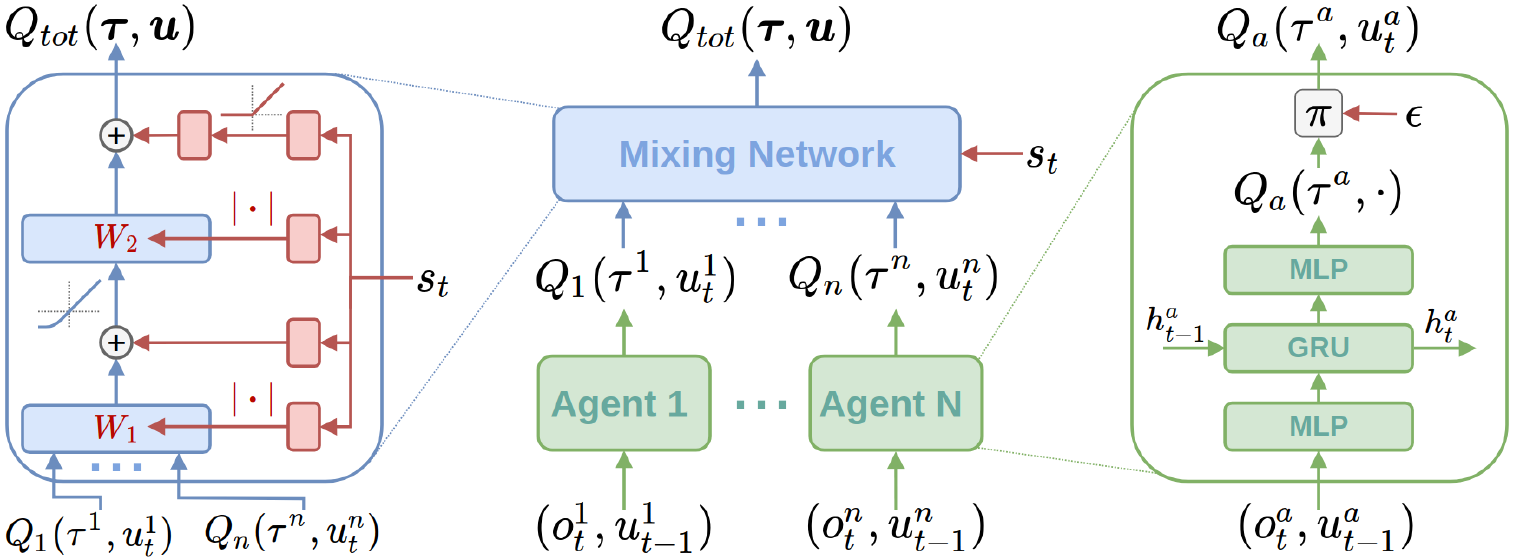
\includegraphics[width=0.8\linewidth]{Figures/MADRL/qmix.png}
    \caption{The architecture of QMIX~\citep{Rashid2018_QMIX} illustrating the learnt monotonic value factorisation. The middle shows the overall architecture with local action-value functions, mixed in to compute the joint action-value. On the left is shown the mixing network that takes in the local action-values to compute the joint action-value, with the weights generated by the hypernetwork (in red) conditioned on the global state. On the right, the architecture for a local action-value function is described, with a recurrent network (GRU) used for memory.}
    \label{fig:QMIX}
\end{figure}



\subsection{Differentiable Emergent Communication}\label{sec:MADRL:EmergentCommunication}

\begin{figure}
    \centering
    \begin{subfigure}[b]{0.88\textwidth}
        \centering
        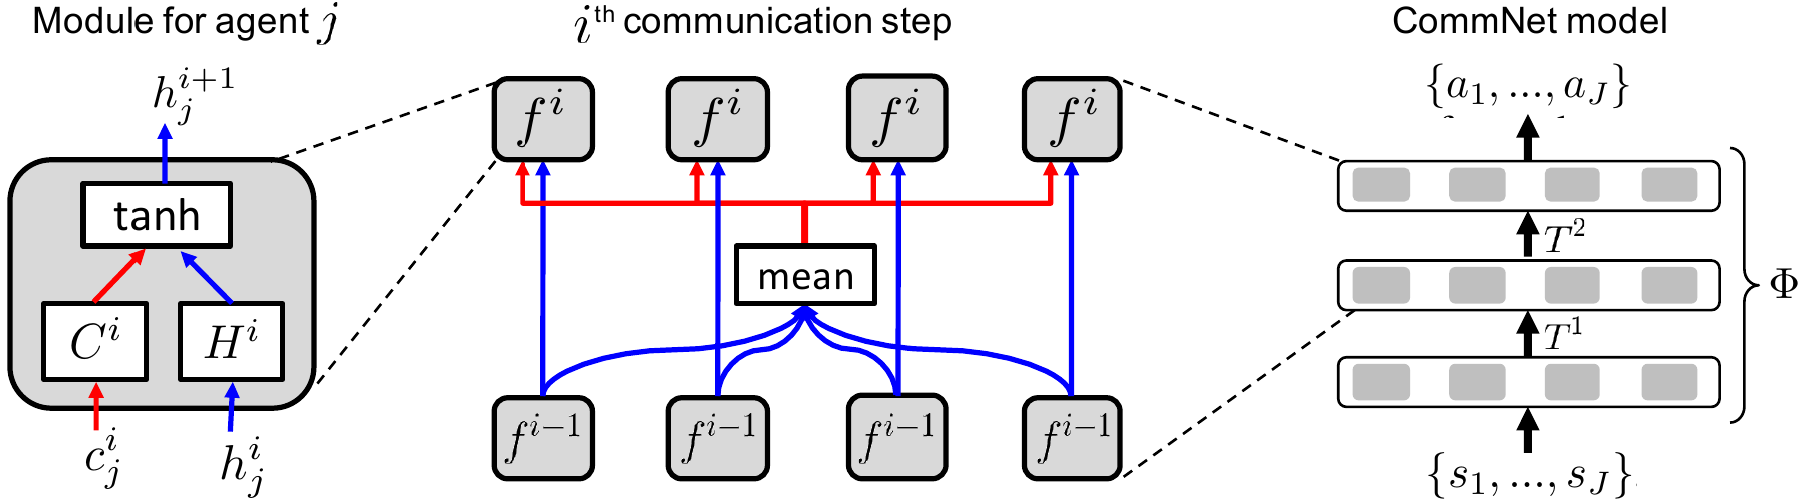
\includegraphics[width=\textwidth]{Figures/MADRL/commnet.png}
        \caption{CommNet~\citep{Sukhbaatar2016_CommNet}}
        \label{fig:CommNet}
    \end{subfigure}
    \begin{subfigure}[b]{0.52\textwidth}
        \centering
        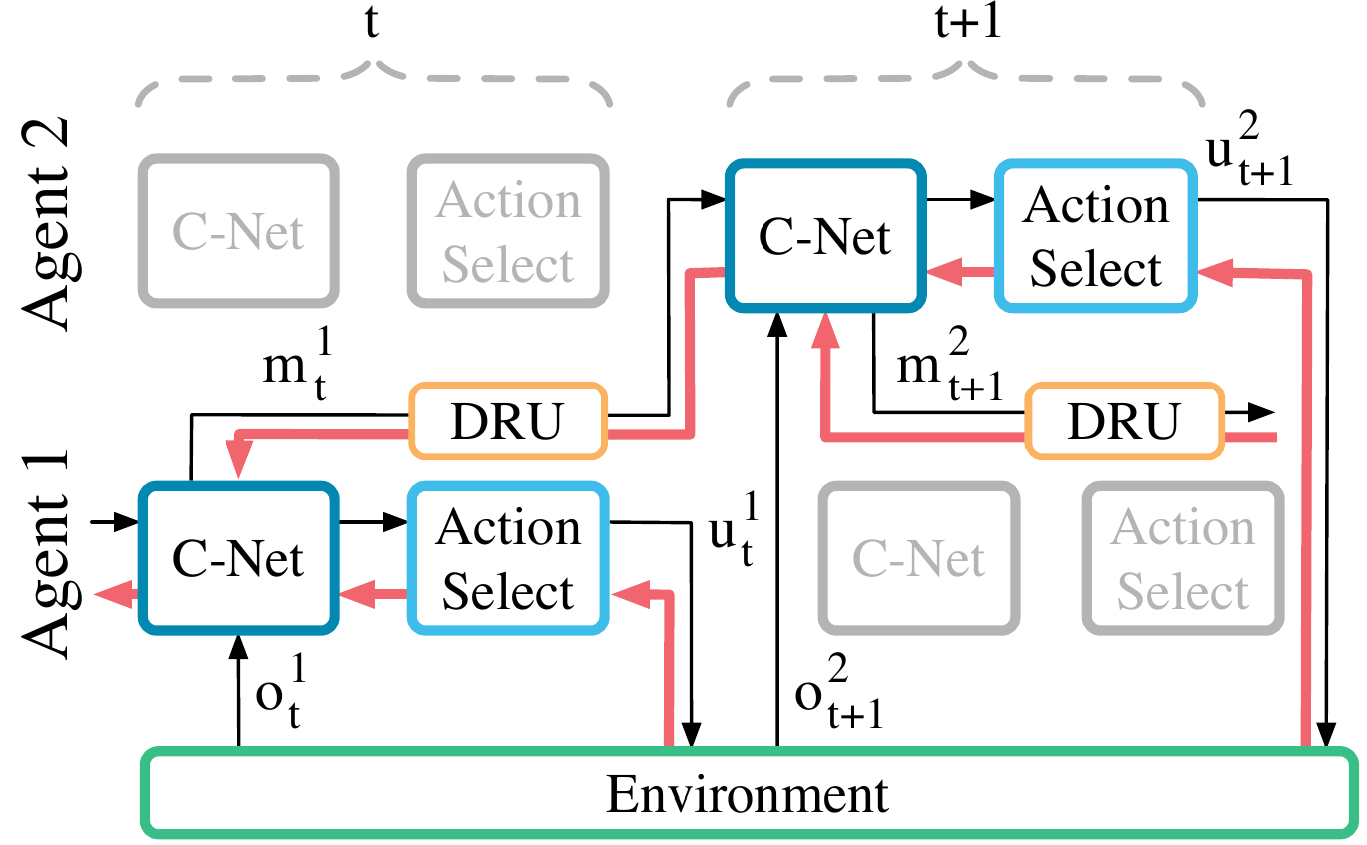
\includegraphics[width=\textwidth]{Figures/MADRL/dial.png}
        \caption{DIAL~\citep{Foerster2016_DIAL}}
        \label{fig:DIAL}
    \end{subfigure}
    \caption{Two architectures of differentiable communication. (a) CommNet learns a centralised communication network that shares local information in multiple rounds of communication before choosing local actions. (b) DIAL learns decentralised communication with centralised training, by allowing gradients to flow between agents. Because messages result from differentiable operations of neural networks, communication can emerge from back-propagation of gradients from the RL objective.}
\end{figure}

An important part of human interactions is communication. We often use our multi-modal communication abilities (e.g., speech, language, hand gestures, facial expressions) to share our knowledge, coordinate our actions, negotiate, or express goals and feelings. It is therefore natural to study communication in the context of multi-agent learning. We have seen, in Section~\ref{sec:MAL_issues}, that the decentralised aspect of multi-agent settings gives rise to many issues that can be alleviated with efficient multi-agent communication. To achieve this, agents need to learn how to communicate. This may be summarised as learning \textit{what to communicate} and \textit{how to communicate it}. A popular approach for learning communication in a multi-agent setting is to let agents develop their own communication system in the process of learning to complete a given task. This gives rise to an emergent communication system that specifically fills the communication needs of the task. 

% Differentiable communication
Recently, a successful approach to emergent communication with MADRL has been to implement communication as a differentiable sub-step of the action-selection process~\citep{Sukhbaatar2016_CommNet, Foerster2016_DIAL}. By using only differentiable operations -- i.e., neural networks -- to generate and process the messages, the gradients of the RL objective can be back-propagated through the message-generating modules so they participate in maximising future returns. Importantly, having differentiable messages allows for gradients to be passed between agents: as a message generated by agent $i$ will impact the choices made by agent $j$, agent $i$ can be trained to generate messages that maximise agent $j$'s returns. This way, the communication mechanisms emerge from the task requirements. CommNet~\citep{Sukhbaatar2016_CommNet} introduced a centralised approach of differentiable communication (see Figure~\ref{fig:CommNet}), with all agents sharing a communication network enabling information sharing and trained to maximise the joint return. DIAL~\citep{Foerster2016_DIAL} took this into the CTDE paradigm (see Figure~\ref{fig:DIAL}), with each agent's communication network (C-Net in the figure) trained from the other agent's learning objective. In these two approaches, neural networks generate differentiable messages comprised of a vector of continuous values, which may carry information to other agents. By learning to maximise the RL objective, the message-generating networks are trained to generate messages that allow other agents to select better actions. 

This approach of differentiable communication has been extended in various ways for more targeted information sharing~\citep{Hoshen2017_VAIN, Jiang2018_ATOC, Das2019_TarMAC} or to limit bandwidth usage~\citep{Singh2019_IC3Net, Zhang2019_VBC, Wang2020_IMAC, Han2023_MBC}. While previously cited works use \textit{continuous vectors} as messages, others have developed techniques to use \textit{discrete symbols} for communicating~\citep{Cao2018_Negotiation, Lazaridou2018_Emergence, Jaques2019_SocialInfluence, Kim2018_SchedNet, Rita2022_GenOverf}. Discrete symbols are advantageous because they limit the bandwidth of transmitted messages. They also incite the emergence of certain qualities of natural languages that make human communications so efficient~\citep{Mordatch2018_GroundedCompo, Chaabouni2019_AntiEfficient}. 

% problem with emergent comm, quick word on grounding and ref to chap 4
While emergent communication allows efficient learning of information transmission with deep RL, it has important limitations. As with all deep learning approaches, it acts as a black box that lacks practical ways of interpreting and measuring its efficiency~\citep{Lowe2019_Pitfalls, Lazaridou2020_DeepEmergentComm}. Because it emerges from task-oriented training in a closed group of agents, the resulting communication mechanism will be hardly usable for solving different tasks and communicating with other agents. For these reasons, methods are investigated to learn more interpretable and generalisable communication skills. In Chapter~\ref{ChapterComm}, we will look into communication and language more in depth, to see how multi-agent communication can be improved. 





\subsection{Agent Modelling}\label{sec:MADRL:AgentModelling}

% Modelling other agents
Previously presented approaches rely on learning policy and value functions to learn multi-agent behaviour. This model-free approach predominates in multi-agent learning because learning a model in a multi-agent setting is made extremely difficult by the fact that, from one agent's perspective, other agents contribute to the environment dynamics: the transition probability and reward function. 
One step towards solving this is to learn a model of other agents' policies, based on previous observations~\citep{Albrecht2018_AgentModellingReview}. 
% this is a kind of multi-agent model-based approach, that can enable better planning or solving multi-agent issues such a scredit assignment or non-statio
In fictitious play~\citep{Brown1951_FictitiousPlay,Robinson1951_FictitiousPlay, Fudenberg1995_FictitiousPlay, Hofbauer2002_FictitiousPlay}, each agent keeps track of action counts by other policies to compute potential action probabilities, then choosing an action accordingly. Recent deep RL techniques have been employed to improve fictitious play and allow its use in more complex, partially observable environments~\citep{Heinrich2016_NSFP, Strouse2021_FCP, Papoudakis2021_LIAM, Rahman2023_GPL, Jing2024_OfflineOpponentModel}. 
Bayesian learning goes further by tracking probabilities over possible policies for other agents, allowing to model uncertainty about their current reasoning~\citep{Jordan1991_Bayesian, Kalai1993_Rational, Bowling2001_Rational, Foerster2019_BAD, Hu2020_SAD}. 
Such agent modelling approaches are promising for learning intricate multi-agent interactions, as they allow to adapt to the observed behaviour of other agents instead of trying to learn a policy able to effectively answer to any situation. Additionally, this approach has the intuitive advantage of emulating the way human beings approach their interactions with other intelligent entities, as described by the \textit{theory of mind} literature~\citep{Apperly2011_Mindreaders, Heyes2014_MindReading, Aru2023_DeepLearningToM}. 

% conclusion -> agent modelling is interesting direction, as model-based RL, it can lead to interesting planning abilities and help solving multi-agent problem such as credit assignment or non-statio.

% Raileanu2018_SOM: predict other agents' goals to 
% LOLA uses it to reduce non-statio by considering how other agents will learn, in the learning update
% Kim2021_IS uses it for driving communication

%  ToM?
% LOLA? introduces opponent modelling into learning to reduce non-stationarity, the learning update takes into account the fact that other agents will also change their behaviour.

% - Instead of making decisions based only on expected returns and how they may be maximised by other agents, one could prefer explicetly predict the other agents goals and/or policies based on previous behaviours [Albrecht2018_AgentModellingReview].
% - Fictitious play (A128) [Brown1951_FictitiousPlay,Robinson1951_FictitiousPlay, Fudenberg1995_FictitiousPlay, Hofbauer2002_FictitiousPlay]
%   - Keeps track of action count by each policy to compute probability of each actions, and computes a best response to the modelled policies
%   - improvements with recent deep RL techniques allow to better learn agent models in more complex, partially observable environments [Heinrich2016_NSFP, Strouse2021_FCP, Papoudakis2021_LIAM, Rahman2023_GPL, Jing2024_OfflineOpponentModel]
% - Bayesian learning (A134): 
%   - track probabilities overs possibles policies for other agents, allowing to model the uncertainty of one agent's about the others' policies [Jordan1991_Bayesian,Kalai1993_Rational,Bowling2001_Rational, Foerster2019_BAD, Hu2020_SAD]
% (  - modelling uncertainty enables considering the value of gaining information about other agents when selecting actions [])
% - ? Theory of Mind

%   LOLA!

% REFS A127, Albrecht2018_AgentModelling





% -------------------------------------------------------------------------------------------------

\section{Robotic Perspectives on MADRL Research: Open Challenges and Shortcomings}\label{sec:MADRL_RobotPerspective}

One of the key objectives of MADRL research is to facilitate the integration of robots into our daily lives. The real world is inherently multi-agent, as almost all conceivable situations involve interactions with other intelligent entities. Consequently, MADRL research aims to extend RL algorithms to be applied in complex multi-agent settings that more accurately reflect everyday scenarios. However, despite this objective, the current state of research has not yet come this far. The methods presented in the previous section are hardly applicable to robotic settings without significant modifications. This is partly because these methods are designed to be general multi-agent learning approaches, rather than being specifically designed for robotics. However, it may also result from some inherent limitations in their learning techniques or shortcomings of MADRL research. 

In this section, we present four important challenges faced in MADRL research that must be addressed to enable the progress of MADRL algorithms in robotics. We define these challenges, examine how they are typically addressed, explore specific approaches to overcome them, and discuss potential improvements. While there may be other obstacles to overcome, we believe these challenges represent the main avenues for improving robotic control in complex multi-agent environments. 



\subsection{Benchmarking MADRL}\label{sec:MADRL:Benchmark}

% Many different environments
Rigorous evaluation and comparison of different MADRL methods have been difficult to carry out due to several key challenges. Firstly, there is a large variety of learning environments and tasks, with little consensus on which setting should be used for studying which multi-agent problem. The most frequently found environments are the \textbf{Starcraft multi-agent challenge} (SMAC, see Figure~\ref{fig:SMAC};~\cite{Samvelyan2019_SMAC}) and the \textbf{multi-agent particle environment} (MPE, see Figure~\ref{fig:MPE};~\cite{Lowe2017_MADDPG}), but many others are also studied (see Figures~\ref{fig:madrlenvs}c-f). Most environments have multiple tasks available for training and testing algorithms. But, it is often unclear what multi-agent learning problems are featured in a given task. Thus, different works choose different environments and tasks arbitrarily based on their preferences, available computing power, and the performance of their method. 
This complicates the comparison of different works that tackle different environments and tasks. Additionally, the value and rigour of these environments are seldom questioned, as shown by the recent revision of SMAC after it was found to be solvable by only observing the current time step~\citep{Ellis2023_SMACv2}. 
Some other interesting environments are often proposed, for more efficient computation~\citep{Lechner2023_GigaStep, Michalski2023_SMACLite}, human-agent teaming~\citep{Carroll2019_Overcooked}, for allowing more agents~\citep{Lechner2023_GigaStep}, more various tasks~\citep{Leroy2023_IMPMARL}, or more realistic settings~\citep{Kurach2020_GoogleFoot, Vinitsky2022_Nocturne}; but there are seldom included in new studies and benchmarks. 

% Implementations
Secondly, a thorough comparison with all existing methods is difficult. Learning multi-agent policies generally takes time and computing power. Among the available implementations, multiple versions of the same methods may have slight differences that are not always clearly stated. Different works might use different programming tools. While the programming language Python is widely adopted in Machine Learning, various Python libraries exist for implementing learning algorithms. No single library is universally preferred\footnote{Pytorch (\url{https://pytorch.org/}) is the most used in research, but some still use TensorFlow (\url{https://www.tensorflow.org/}), and a growing number of people prefer JAX for its computational efficiency~\citep{Jax2018}.}, leading to significant differences that prevent easy adaptation from one library to another. 

% In-method discrepancies
Lastly, the implementation of each method may differ from one work to another. All methods come with a very large set of hyperparameters, with some having a great impact on performance. Deep RL methods, which serve as the foundation for MADRL methods, can be implemented differently, with some implementation tricks having a major impact on performance. This variability makes comparison across different studies challenging.

% MADRL envs: SMAC, MPE, LBF, RWARE, Hanabi, magym
\begin{figure}
    \centering
    \begin{subfigure}[c]{0.35\textwidth}
        \centering
        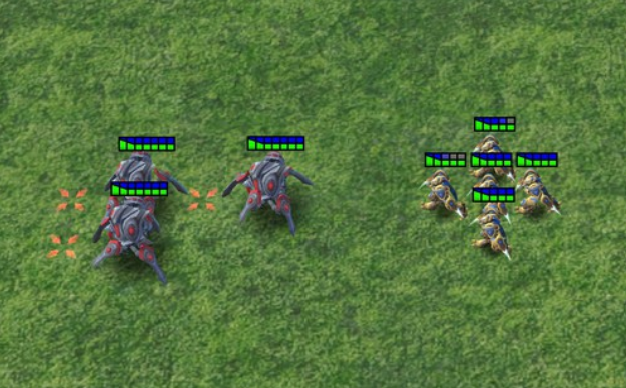
\includegraphics[width=\textwidth]{Figures/MADRL/smac.png}
        \caption{SMAC}
        \label{fig:SMAC}
    \end{subfigure}
    \hfill
    \begin{subfigure}[c]{0.24\textwidth}
        \centering
        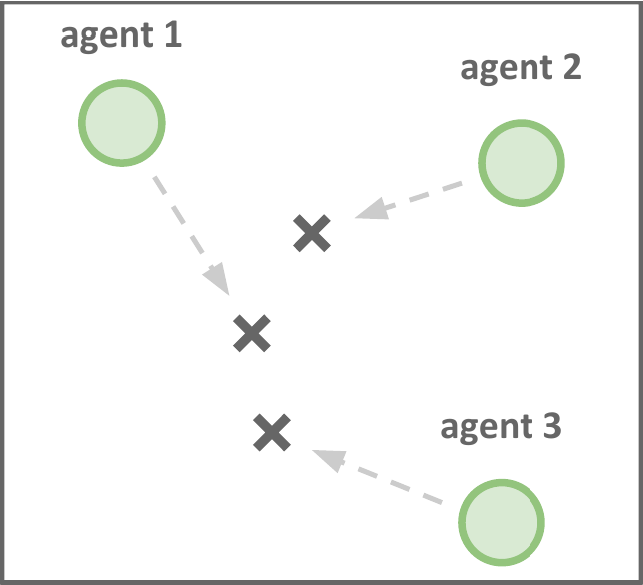
\includegraphics[width=\textwidth]{Figures/MADRL/mpe.png}
        \caption{MPE}
        \label{fig:MPE}
    \end{subfigure}
    \hfill
    \begin{subfigure}[c]{0.225\textwidth}
        \centering
        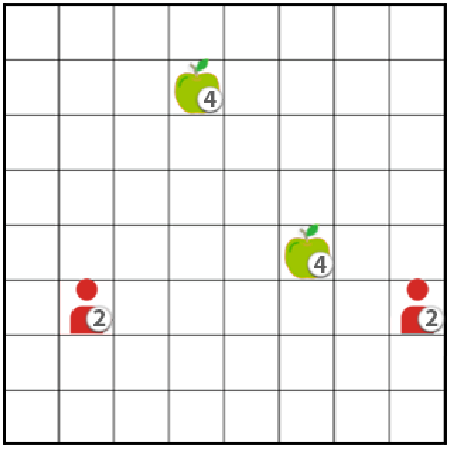
\includegraphics[width=\textwidth]{Figures/MADRL/lbf.png}
        \caption{LBF}
        \label{fig:LBF}
    \end{subfigure}
    
    \begin{subfigure}[c]{0.225\textwidth}
        \centering
        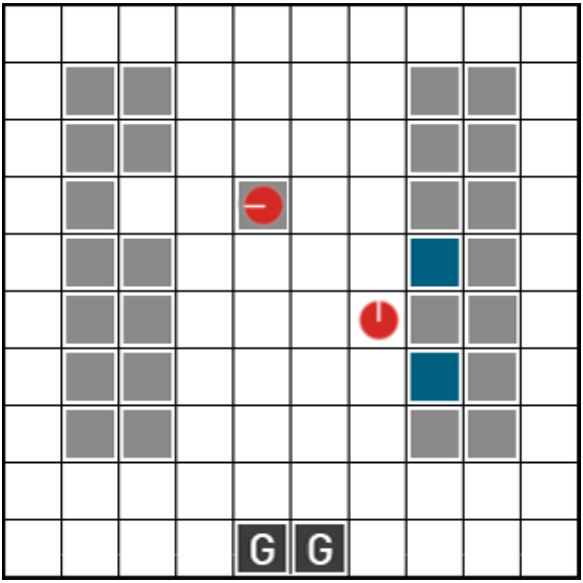
\includegraphics[width=\textwidth]{Figures/MADRL/rware.png}
        \caption{RWARE}
        \label{fig:RWARE}
    \end{subfigure}
    \hfill
    \begin{subfigure}[c]{0.44\textwidth}
        \centering
        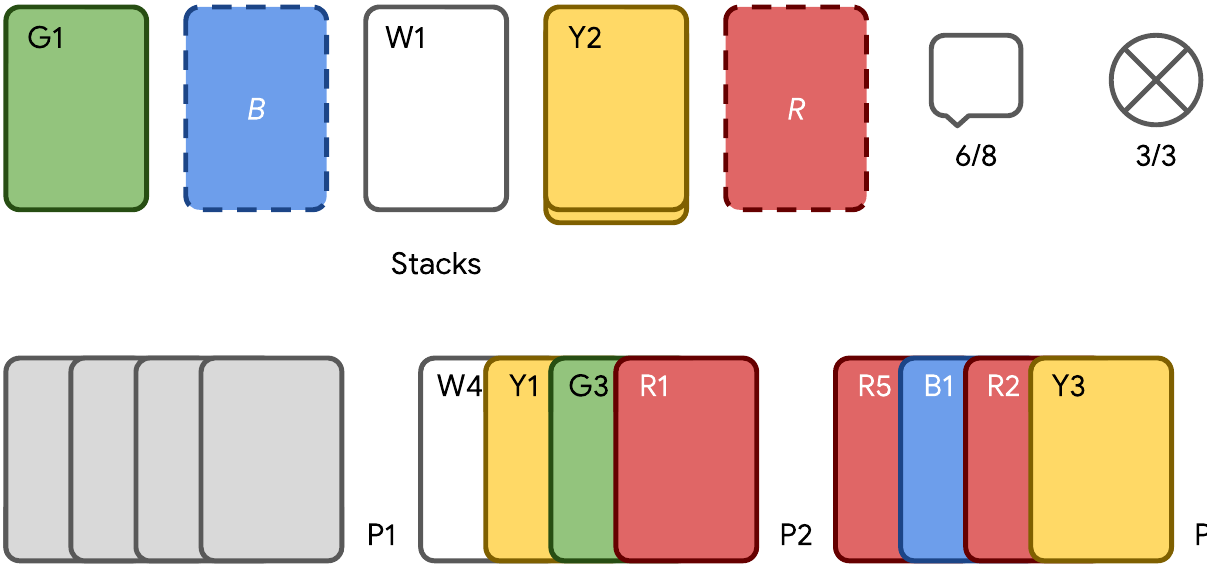
\includegraphics[width=\textwidth]{Figures/MADRL/hanabi.png}
        \caption{Hanabi}
        \label{fig:Hanabi}
    \end{subfigure}
    \hfill
    \begin{subfigure}[c]{0.225\textwidth}
        \centering
        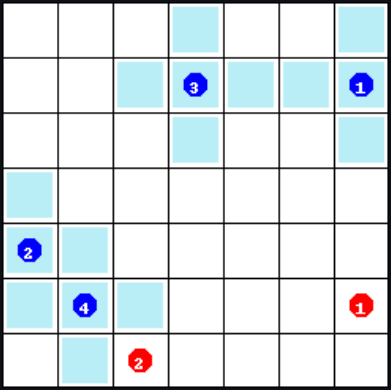
\includegraphics[width=\textwidth]{Figures/MADRL/magym.png}
        \caption{ma-gym}
        \label{fig:magym}
    \end{subfigure}
    \caption{The most used MADRL environments. (a) The \textit{Starcraft multi-agent challenge} (SMAC;~\cite{Samvelyan2019_SMAC}), with teams of units fighting opponents in various scenarios. (b) The \textit{multi-agent particle environment} (MPE;~\cite{Lowe2017_MADDPG}), a two-dimensional continuous environment with various tasks studying cooperative navigation and communication. (c) The \textit{level-based foraging} (LBF;~\cite{Albrecht2013_Foraging}) task, studying coordination in a grid world. (d) The \textit{multi-robot warehouse} (RWARE;~\cite{Christianos2020_SharedExp}), a robotic task in a grid world. (e) The cooperative card game \textit{Hanabi}~\citep{Bard2020_Hanabi} for studying complex team strategy learning and adaptation to teammates. (f) The \textit{ma-gym} two-dimensional grid world environment, with various cooperative tasks.}
    \label{fig:madrlenvs}
\end{figure}

% Benchmarking problem
For these reasons, assessing the progress of MADRL research is difficult. Performance reported in papers is hard to take at face value because of untold discrepancies hidden in the implementations and reported results~\citep{Singh2023_EvalMARL}. For example, \cite{Gorsane2022_BenchmarkCoopMARL} show inconsistencies in the performance of QMIX reported in different papers. The consequence of this lack of standardised benchmark is concerning: it is unclear which methods are the best for any given purpose, and therefore what method should be used as a baseline in any given setting. To advance learning in multi-robot environments, it would be difficult to determine the most valuable MADRL algorithms to use in these environments. 

% Existing benchmarks
Some benchmarks have been presented to try tackling this issue~\citep{Yu2021_Benchmark, Papoudakis2020_BenchmarkMADRL, Ellis2023_SMACv2, Bettini2023_BenchMARL}. They help clarify the field by providing a common ground for comparing important methods. However, there is limited variety in the environments used in these benchmarks, so the results might not hold in other tasks or more complex environments. It is also unclear what exact skill sets are required in each task, with only a rough measure of difficulty based on the returns obtained by all methods. This makes it difficult to discern the specific advantages of each method over others. Nevertheless, there are attempts to propose standardised evaluation protocols for new works~\citep{Gorsane2022_BenchmarkCoopMARL, Singh2023_EvalMARL}, which is a promising avenue for building stronger and more progressive research in MADRL. 

% Better benchmarks
To move forward, better practices should be adopted. Proposed methods should all disclose hyperparameters and specific code-level optimisations. Evaluation protocols and metrics should be standardised across all new publications~\citep{Gorsane2022_BenchmarkCoopMARL}. Benchmarks should include more diverse environments, integrating the wide range of potential learning problems studied across multi-agent learning: continuous and discrete settings, various degrees of centralisation allowed during training and execution, communication between agents, and different degrees of environmental complexity with environments closer to robotics. There is no doubt that MADRL research would immensely benefit from improving its evaluation protocols as such, allowing less biased comparison between methods and deeper analysis of their abilities. This is essential for efficiently advancing the field and ensuring that proposed methods are robust and generalisable across tasks and environments. 





\subsection{Exploration}

% The problem
Exploration is arguably one of the most important problems in single-agent RL~\citep{Hao2024_ExploReview}. It is particularly crucial when dealing with sparse rewards, where only a few interactions in the environment yield positive reinforcement signals. Such settings are often termed "hard-exploration" problems, requiring techniques allowing consistent discovery of the infrequent rewarding states.
In multi-agent RL, the problem is exacerbated. Performance depends on the joint behaviour of all agents, requiring exploration of the space of joint policies to identify the best approaches. Exploration becomes a multi-agent problem, especially when coordination is necessary, as agents need to explore different ways to act in unison. 
Exploration is also a major subject in robotic environments. Partial observability complicates the issue, as one environment state may be observed from many different perspectives. Moreover, the safety concerns are both a constraint and an expectation for exploration. When exploration is conducted on robots, it should only involve safe states to ensure that robots do not injure themselves or others~\citep{Koller2018_MBCSafeExp, Ding2021_SafeExp}. At the same time, exploration is a way to find the optimal strategies that are safer for the robots. In this sense, exploration might be conducted in simulation to identify safe behaviours to execute on physical robots~\citep{Garcia2015_SafeRL, Brunke2022_SafeLearningRobots}. 

% How methods explore
Most single and multi-agent RL approaches treat exploration arbitrarily by infusing randomness into the behavioural policy during training. Q-learning-based approaches employ the epsilon-greedy strategy (see Section~\ref{sec:RL:Qlearning}), policy-based approaches either add noise to actions, as seen in DDPG, or maximise the entropy of the policy, as in PPO (see Section~\ref{sec:DRL:Policy}). However, these methods are often insufficient for dealing with hard exploration problems~\citep{Ostrovski2017_PseudoCounts, Pathak2017_ICM, Burda2019_RND}. In multi-agent environments, random exploration often leads to the problem of relative overgeneralisation, where agents are attracted towards suboptimal Nash equilibria because the optimal strategy is too marginal to be found consistently through random exploration~\citep{Wiegand2003_RelOvergen}. 
In Chapter~\ref{ChapterJIM}, we will tackle this issue of multi-agent exploration by describing the problem of \textit{relative overgeneralisation} that results from poorly coordinated exploration, reviewing the related literature, and exploring intrinsic motivation to explicitly induce joint exploration. 




\subsection{Generalisation}\label{sec:MADRL:Generalisation}

Generalisation is a significant problem in machine learning and single-agent RL, concerning the robustness of learnt models to situations unseen during training. In RL, this may correspond to different initial conditions or new environmental settings. A good model is one that maintains its training performance in these new situations. In the multi-agent setting, the problem persists and even evolves with multiple agents, requiring to handle changes in the strategies of other agents. 

In machine learning, good generalisation is typically achieved through extensive training on very large amounts of data. However, this becomes challenging when faced with embodiment issues (see Section~\ref{sec:MAL:Embodiment}). In RL, the training data is generated by the agents themselves. Thus, in multi-agent RL, acquiring a comprehensive understanding of the joint policy space is a challenging exploration problem, as discussed in the previous section. In multi-agent RL, agents usually train in "self-play", with a fixed team of agents learning by trying to solve the task together. However, this often leads to agents converging to an arbitrary convention on collective behaviour, which may not hold with new partners. This is a problem in robotic settings, where the environment is dynamic and robots are expected to efficiently and safely handle new robotic or human partners. 

Generalising to new environmental situations can be facilitated by having diverse environmental settings, such as procedural maps, which allow training in many different scenarios and, hopefully, learning more general policies~\citep{Jaderberg2018_FTW, Cobbe2020_ProcGen}. For generalising to different partners, one approach is population-based training, involving a large number of agents trained in dynamic teams to face various strategies during training~\citep{Jaderberg2018_FTW, Liu2019_CoordThroughComp, Zhao2023_MaxEntropPop}. While this can be very effective~\citep{Jaderberg2018_FTW}, it requires extensive training sessions to converge to general strategies. This may be impractical in high-dimensional and dynamic robotic environments, where training is expensive and accounting for all possible modifications of a real environment is impossible. Moreover, if humans are involved, it is impossible to train for all possible changes in human behaviour. 

A promising approach is to learn to quickly adapt to any situation. In single-agent RL, \textit{zero-shot generalisation} methods aim to adapt to unseen environmental settings without being retrained~\citep{Kirk2023_ZeroShotGene, Haarnoja2024_Soccer}. In multi-agent RL, this concept extends to zero-shot, or \textit{ad hoc}, teaming, where agents are evaluated with new partners~\citep{Stone2010_AdHocTeam}. Agent modelling is promising for such settings, allowing to learn to model the "type" of policy observed in other agents~\citep{Strouse2021_FCP, Xie2021_LILI, Rahman2023_GPL, Yan2023_E3T}, or even the exact agents faced~\citep{Barrett2017_MakingFriends, Lanctot2023_RockPaperScissors}, allowing better reactions to the observed behaviour. If learned properly, zero-shot teaming can be a valuable tool for human-agent teaming. Training with humans is expensive, so it may be more efficient to learn to adapt quickly to any human partner~\citep{Strouse2021_FCP, Shih2021_ConventionsHumanAI, Xie2021_LILI, Yu2023_HiddenUtilitySP, Yan2023_E3T}. 



% \subsection{Decentralisation}

% while centralised methods were popular in earlier MARL research, recent research shifts to more decentralisation
% (as shown in figure ?)
% ctde is a step
% but training would also benefit from being more decentralised
% for scaling to larger number of agents. many robotic applications are not limited in the number of robots or other intelligent entities. ctde methods that use centralised observations during training
% for learning on robots, 
% for continuous learning 

% Human-robot interaction
\begin{figure}
    \centering
    \begin{subfigure}[c]{0.41\textwidth}
        \centering
        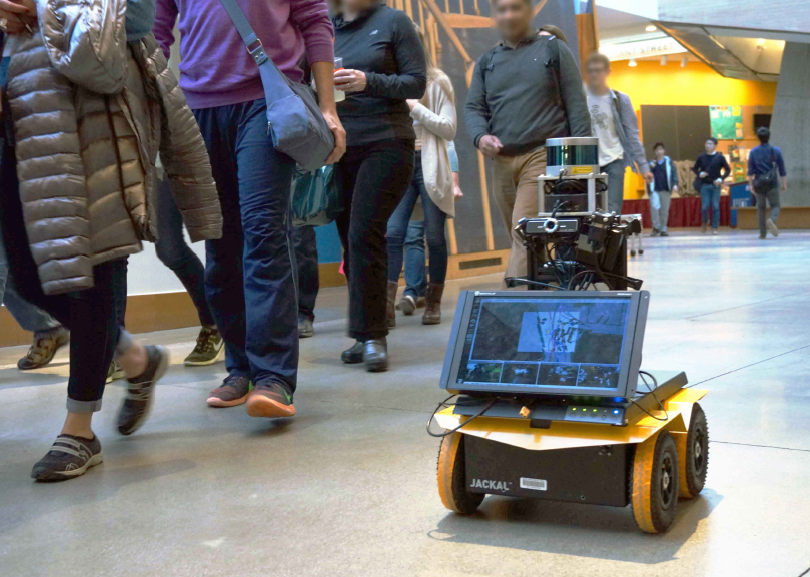
\includegraphics[width=\textwidth]{Figures/MADRL/robnav.png}
        \caption{}
        \label{fig:robnav}
    \end{subfigure}
    \hfill
    \begin{subfigure}[c]{0.39\textwidth}
        \centering
        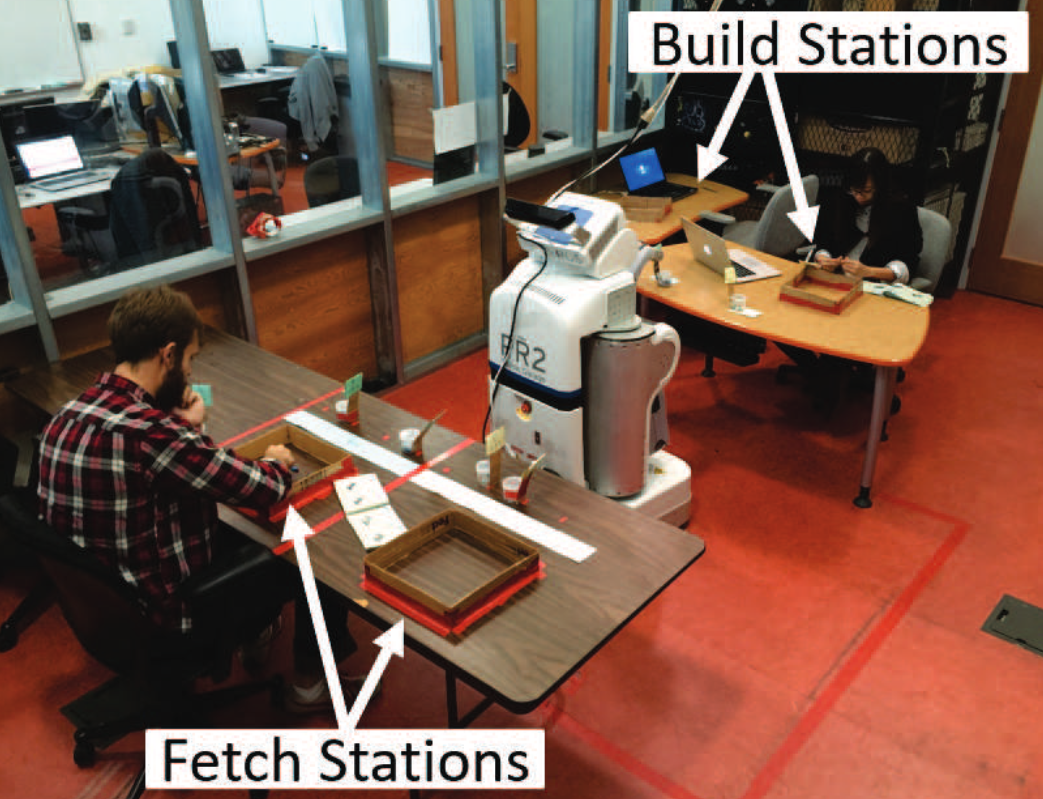
\includegraphics[width=\textwidth]{Figures/MADRL/robassist.png}
        \caption{}
        \label{fig:robassist}
    \end{subfigure}
    
    \begin{subfigure}[c]{0.36\textwidth}
        \centering
        
\includegraphics[width=\textwidth]{Figures/MADRL/robsocial.png}
        \caption{}
        \label{fig:robsocial}
    \end{subfigure}
    \caption{Examples of human-robot interaction. (a) Navigation of a robot in a human-populated environment~\citep{Chen2017_CollisionAvoidance}. (b) A robot assisting humans in a building task by fetching objects~\citep{Gombolay2017_MixedInitiative}. (c) A robot helping a child with autism spectrum disorder to learn social interaction~\citep{Scassellati2018_ASDRobot}.}
    \label{fig:HRI_examples}
\end{figure}

\subsection{Interaction}\label{sec:MADRL:Interaction}

Having robots in real environments implies the need for handling interactions with human beings. Figure \ref{fig:HRI_examples} shows different examples of human-robot interaction (HRI), illustrating various levels of HRI with differing degrees of connection between robots and humans, ranging from simply living in a human-populated environment to deep social interactions between robots and humans. Across all these potential scenarios, we can identify three sub-problems of HRI. First, to enable interaction between humans and computer systems in general, we need to understand how humans behave. This means studying how they go about solving a task, to know how robots could help them and how they should not~\citep{Shih2021_ConventionsHumanAI}. This means understanding how they interact with each other, to understand what makes a successful human interaction and how robots could be a part of them~\citep{Tseng2016_ServiceRobot}. This also means studying how humans react to robots when they interact with them, to understand the differences between human-human and human-robot interactions~\citep{Jung2020_TowerConstruct, Roesler2024_HumanRobotTrust}. And, this means studying how humans communicate with each other, investigating different tools like natural language, body language, and a large variety of social cues~\citep{Feine2019_SocialCues}. 
Analysing how humans behave in social interactions and when cooperating to fulfil a task can help design better robots and more effective learning approaches for HRI.

Second, HRI requires designing proper interfaces to enable smooth interactions. This involves physical interfaces, including the ability to sense, grasp, move, point and look at particular objects. These physical abilities are not needed only for interacting with human beings, but the HRI component might influence the design of these skills. Social interfaces are also required, with the help of human-like features such as voice, eyes, articulated faces, and gestures~\citep{Zlotowski2014_Anthropomorphism}. Being able to communicate with humans is also an important requirement to allow information sharing, teaching, strategy evaluation and correction~\citep{Mikolov2018_RoadmapMachineIntell, Crandall2018_CoopWithMachines}, and, more generally to bond more easily with artificial agents~\citep{Liu2022_ChildChatbotReading}. In Chapter~\ref{ChapterComm}, we will explore in greater depth the role of communication and language for human-agent interaction. 

Finally, HRI requires learning to behave around humans and cooperate with them. This is where MADRL research becomes relevant, as it enables learning in complex environments with multiple intelligent entities interacting. However, the main MADRL algorithms, discussed in Section~\ref{sec:MADRL_Review}, are not specifically intended for interacting with humans. They need to be extended using various techniques to efficiently address the problems linked with embodiment (see Section~\ref{sec:MAL:Embodiment}). The generalisation problem, described previously, must be tackled to enable robots to interact with any given human partner. And, to enable the use of MADRL algorithms on real robots, we need efficient approaches for bridging the reality gap (see Section~\ref{sec:MAL:RealityGap}). 





% -------------------------------------------------------------------------------------------------

\section{Conclusion}\label{sec:MADRL_Conclusion}

This chapter explored the domain of MADRL research, from the perspective of robotics. One of the objectives of MADRL research is to learn behavioural policies for controlling robots in the real world. Thus, it is important to reflect on the current state of progress in this domain, analyse the relevance of recent studies for robotics, and see how the challenges of robotic environments are addressed. After formally defining the tools of MADRL, we have presented the main challenges faced in multi-agent learning and robotics. Some of these challenges are specific to one of the two areas, but many overlap on many aspects. This analysis shows that connecting these two domains means dealing with many different forms of complexity, in environmental settings, interactions, and unpredictable situations. 

In Section~\ref{sec:MADRL_Review}, we presented a survey of the main avenues of MADRL research, describing how state-of-the-art methods learn policies in multi-agent settings. While some techniques have been shown to tackle increasingly complex tasks and environments, the main approaches are still far from being applicable in a robotic scenario without significant adaptation. This can be attributed to the fact that MADRL research is focused on the optimisation problem of multi-agent learning, i.e., finding an efficient multi-agent strategy. Doing so, it often overlooks some problems faced in realistic scenarios and thus fails to progress towards more efficient learning algorithms. 

In Section~\ref{sec:MADRL_RobotPerspective}, we introduced multiple challenges for MADRL research that should be addressed for improving the field, especially for moving towards robotic applications. The benchmarking issue faced in the domain is especially important to solve rapidly to ensure a more reliable research field and more steady progress. Next, the problems of exploration, generalisation, and interaction, are all key to improving the efficiency and applicability of new MADRL algorithms. We believe these challenges represent the main directions for advancing the control of robots in complex multi-agent environments, and that MADRL algorithms would benefit from investigating them further. 

Following this analysis of MADRL algorithms, in the next chapters, we propose two new methods for tackling some of the challenges defined previously. First, in Chapter~\ref{ChapterJIM}, we investigate the problem of exploration further, by highlighting the weaknesses of existing MADRL algorithms and proposing a method for improving them by exploring in a coordinated fashion. Next, in Chapter~\ref{ChapterComm}, we tackle the problem of communication in multi-agent systems, and propose an algorithm for learning to communicate with a pre-defined language which, as we demonstrate, serves multiple purposes of the robotic setting. 